% !TEX root = main_usenix_style_round3_clean.tex
\documentclass[letterpaper,twocolumn,10pt,twoside]{article}

\usepackage[
  letterpaper,
  top=0.75in,
  bottom=1.00in,
  left=0.75in,
  right=0.75in,
  columnsep=0.25in
]{geometry}
\usepackage{fontspec}
\defaultfontfeatures{Ligatures=TeX}
\setmainfont{Times New Roman}
\setsansfont{Arial}
\setmonofont{Courier New}
\usepackage{microtype}
\usepackage{graphicx}
\usepackage{booktabs}
\usepackage{multirow}
\usepackage{array}
\usepackage{amsmath}
\usepackage{amssymb}
\usepackage{enumitem}
\usepackage{caption}
\usepackage{subcaption}
\usepackage{fancyhdr}
\usepackage{placeins}
\usepackage{url}
\usepackage[hidelinks]{hyperref}

\setlist[itemize]{leftmargin=*,topsep=2pt,itemsep=1pt}
\setlist[enumerate]{leftmargin=*,topsep=2pt,itemsep=1pt}
\captionsetup{font=small,labelfont=bf,labelsep=colon,justification=centering,skip=3pt}
\captionsetup[figure]{name=Figure,position=bottom}
\captionsetup[table]{name=Table,position=top}
\setlength{\parindent}{1em}
\setlength{\parskip}{0pt}
\setlength{\textfloatsep}{8pt plus 2pt minus 2pt}
\setlength{\floatsep}{6pt plus 2pt minus 2pt}
\setlength{\intextsep}{6pt plus 2pt minus 2pt}
\setlength{\dbltextfloatsep}{8pt plus 2pt minus 2pt}
\setlength{\dblfloatsep}{6pt plus 2pt minus 2pt}
\flushbottom
\hbadness=10000
\vbadness=10000
\hyphenpenalty=10000
\exhyphenpenalty=10000
\emergencystretch=3em
\setcounter{topnumber}{4}
\setcounter{bottomnumber}{2}
\setcounter{totalnumber}{6}
\renewcommand{\topfraction}{0.97}
\renewcommand{\bottomfraction}{0.90}
\renewcommand{\textfraction}{0.03}
\renewcommand{\floatpagefraction}{0.74}
\renewcommand{\dbltopfraction}{0.97}
\renewcommand{\dblfloatpagefraction}{0.74}
\makeatletter
\setlength{\@fptop}{0pt}
\setlength{\@fpsep}{11pt}
\setlength{\@fpbot}{0pt plus 1fil}
\makeatother
\pagestyle{fancy}
\fancyhf{}
\renewcommand{\headrulewidth}{0pt}
\renewcommand{\footrulewidth}{0pt}
\setlength{\footskip}{34pt}
\newcommand{\usenixfooterfont}{\normalfont\fontsize{9}{10}\selectfont}
\fancyfoot[LO]{}
\fancyfoot[RO]{\usenixfooterfont \thepage}
\fancyfoot[LE]{}
\fancyfoot[RE]{\usenixfooterfont \thepage}

\makeatletter
\renewcommand{\maketitle}{%
  \twocolumn[{%
    \begin{@twocolumnfalse}
      \vspace*{0.80in}
      \begin{center}
        {\Large\bfseries \@title \par}
        \vskip 1.45em
        {\large \@author \par}
      \end{center}
      \vspace{0.14in}
      \begin{center}
        \begin{minipage}{0.92\textwidth}
          \begin{center}
            {\large\bfseries Abstract}
          \end{center}
          \vspace{-0.55em}
          \paperabstract
          \par\vspace{0.75em}
          \noindent\textbf{Keywords:} \paperkeywords
        \end{minipage}
      \end{center}
      \vspace{0.10in}
    \end{@twocolumnfalse}
  }]%
}
\renewenvironment{abstract}{%
  \begin{center}
    {\large\bfseries Abstract}
  \end{center}
  \vspace{-0.55em}
  \noindent
}{\par\vspace{0.75em}}
\renewcommand\section{\@startsection{section}{1}{\z@}%
  {2.0ex plus .6ex minus .2ex}{.8ex plus .2ex}%
  {\normalfont\large\bfseries}}
\renewcommand\subsection{\@startsection{subsection}{2}{\z@}%
  {1.7ex plus .5ex minus .2ex}{.6ex plus .2ex}%
  {\normalfont\normalsize\bfseries}}
\renewcommand\subsubsection{\@startsection{subsubsection}{3}{\z@}%
  {1.4ex plus .4ex minus .2ex}{.5ex plus .2ex}%
  {\normalfont\normalsize\bfseries}}
\makeatother
\newcolumntype{L}[1]{>{\raggedright\arraybackslash}p{#1}}
\newcolumntype{R}[1]{>{\raggedleft\arraybackslash}p{#1}}
\newcolumntype{C}[1]{>{\centering\arraybackslash}p{#1}}
\newcounter{algorithm}
\newsavebox{\algbox}
\newenvironment{algorithmblock}[1]{%
  \refstepcounter{algorithm}%
  \par\medskip\noindent\begin{lrbox}{\algbox}\begin{minipage}{0.94\columnwidth}
  \small
  \textbf{Algorithm \thealgorithm: #1}\par
  \vspace{2pt}\hrule\vspace{3pt}
}{%
  \vspace{2pt}\hrule
  \end{minipage}\end{lrbox}\fbox{\usebox{\algbox}}\par\medskip
}
\newcommand{\alginput}[1]{\noindent\textbf{Input:} #1\par}
\newcommand{\algoutput}[1]{\noindent\textbf{Output:} #1\par}
\newenvironment{algsteps}{\begin{enumerate}[label=\arabic*:,leftmargin=1.8em,itemsep=1pt,topsep=2pt]}{\end{enumerate}}
\newcommand{\tool}{EaTVul-style code insertion evasion attack}
\newcommand{\gate}{sample-level gate}
\newcommand{\Gate}{Sample-level gate}
\newcommand{\windowdef}{window-level diagnostic deletion test}
\newcommand{\Windowdef}{Window-level diagnostic deletion test}
\newcommand{\componentdef}{AST-token component diagnostic deletion test}
\newcommand{\Componentdef}{AST-token component diagnostic deletion test}
\newcommand{\cleanf}{Clean F1}
\newcommand{\asr}{Attack Success Rate (ASR)}
\newcommand{\asrshort}{ASR}
\newcommand{\dataset}[1]{\textsc{#1}}

\title{\Large Detection, Not Sanitization: Capability Boundaries of AST-token-only Defenses against EaTVul-style Code Insertion}
\author{
  Kang Xie\\
  University of South China, Hengyang 421001, Hunan, China\\
  Corresponding author: \href{mailto:q1131714258@gmail.com}{q1131714258@gmail.com}
}
\date{}
\newcommand{\paperabstract}{%
Practical vulnerability-detection deployments often operate through limited artifacts. In third-party scanning, supply-chain auditing, artifact-only benchmarking, and security triage, a defender may observe serialized abstract-syntax-tree (AST) token sequences and detector outputs, but not source spans, source diffs, exact insertion boundaries, control-flow graphs (CFGs), or program dependence graphs (PDGs). This paper studies what remains defensible in that public-artifact setting for EaTVul-style insertion evasion, where inserted code preserves the original vulnerability while shifting the detector toward a benign prediction. We separate deployable review routing from diagnostic deletion tests. Sample-level detection and quarantine ask whether suspicious benign predictions should be automatically accepted; fixed-window and approximate AST-token component deletion ask whether token-only evidence supports recovery. Under a 10\% clean review-routing budget, project-coherent rows reduce automatically accepted benign bypasses substantially: the residual silent-bypass rate is 0.120 on \dataset{OPENSSL} and 0.360 on \dataset{ASTERISK}. Mixed-source transfer is weaker. In contrast, the evaluated deletion tests do not provide sufficient evidence for reliable automatic sanitization because token removal cannot validate source-level boundaries, preservation, or deletion precision. These results support AST-token-only suspicious benign prediction detection and quarantine under project-coherent calibration, but not deployable source-level recovery. For artifact-only vulnerability-detection services, the practical endpoint is review routing rather than unsupported source repair.
}
\newcommand{\paperkeywords}{software vulnerability detection; adversarial code attacks; AST-token defense; quarantine; public-artifact security.}

\begin{document}
\maketitle

\FloatBarrier

\section{Introduction}
\subsection{Background and Motivation}
Learning-based vulnerability detectors are increasingly used to prioritize security review in large software projects \cite{li2018vuldeepecker,zhou2019devign,fu2022linevul,feng2020codebert,guo2021graphcodebert}. In research settings, these detectors are often discussed together with rich program representations: source code, abstract syntax trees (ASTs), data-flow signals, control-flow graphs, and program dependence graphs. Practical deployment can be much narrower. In a third-party software-as-a-service (SaaS) vulnerability-detection service, users may submit tokenized features or exported model artifacts while withholding complete source code. In open-source component supply-chain auditing, a defender may recover serialized AST-token sequences from build artifacts or intermediate representations but lack authoritative source edits. A shared benchmark or artifact-only evaluation may similarly expose only an exported token sequence and a model score. The defender may not receive source locations, edit boundaries, source diffs, CFGs, or PDGs. This gap between research-visible context and deployment-visible artifacts changes the defense problem.

Existing work has mainly advanced two adjacent lines of inquiry. One line builds stronger vulnerability detectors with sequence, transformer, or graph representations \cite{li2018vuldeepecker,zhou2019devign,fu2022linevul,feng2020codebert,guo2021graphcodebert}. Another line studies adversarial code transformations that preserve vulnerable behavior while changing the model input, including identifier renaming, dead-code or snippet insertion, syntax-preserving edits, obfuscation, and EaTVul-style evasion \cite{yefet2020adversarial,chen2022natural,zhou2023advulcode,ramakrishnan2020adversarial,liu2024eatvul}. These directions are important, but they do not fully answer a deployment question: when the defender cannot inspect the original program context, which defensive actions are still justified? In particular, an artifact-only defender may be able to flag a suspicious input but may not be able to locate, delete, or validate the inserted code that caused the evasion.

This question matters for information security applications because artifact-only vulnerability scanning systems must decide whether a benign prediction can be trusted automatically. A silent false negative can remove a real vulnerability from the review queue, even though the original vulnerable behavior remains. When source-aware repair evidence is unavailable, quarantine and review routing provide a more defensible deployment action than automatic relabeling or deletion. The problem studied here is therefore a security deployment boundary, not merely an optimization problem for another machine-learning classifier.

We address this observation-constrained defense question: under the current public EaTVul artifacts, what defensive actions remain justified when the defender has only serialized AST-token sequences? The strict setting considered here gives the defender serialized AST tokens and detector outputs, but not source spans, source diffs, exact insertion boundaries, CFGs, or PDGs. Under this constraint, we ask how far three capabilities can go: detection, which identifies suspicious benign predictions; quarantine, which prevents those predictions from being automatically accepted; and automatic sanitization, which attempts to delete inserted code and recover the vulnerable prediction. The goal is not to propose a complete, general, deployable automatic defense system. Instead, the paper studies the capability boundary of AST-token-only defenses against EaTVul-style insertion evasion.

The main finding is a conditionally asymmetric capability boundary. Detection and quarantine remain feasible under project-coherent settings because inserted code can leave whole-sample distributional and structural traces, whereas mixed-source datasets show weak transfer. Reliable automatic sanitization was not achieved by the evaluated token-only methods, which lack source spans, exact insertion boundaries, syntax validation, control-flow reachability, and dependence relationships. Fig.~\ref{fig:attack-defense-example} summarizes this setting. The paper therefore contributes a boundary analysis for AST-token-only defense and derives a practical recommendation: use public token artifacts to detect and quarantine suspicious benign predictions under project-coherent calibration, but treat automatic sanitization as unreliable unless richer program context is available.

To avoid overextending the empirical claims, we state the scope explicitly. The evidence supports AST-token-only suspicious benign prediction detection and quarantine under project-coherent calibration. It does not support broad transfer to all mixed-source settings, reliable automatic sanitization, or adaptive robustness. The CodeBERT-base experiment is used only as a bounded model-coverage sanity check rather than as broad neural-model evidence.

\begin{center}
  \captionsetup{type=figure}
  \centering
  \setlength{\fboxsep}{5pt}
  \fbox{%
  \begin{minipage}{0.94\columnwidth}
  \scriptsize
  \setlength{\tabcolsep}{3pt}
  \renewcommand{\arraystretch}{1.14}
  \begin{tabular}{@{}L{0.34\columnwidth}L{0.56\columnwidth}@{}}
  \textbf{Available evidence} & Serialized AST-token sequence and detector output. \\
  \midrule
  \textbf{Feasible capability} & Sample-level detection of suspicious benign predictions. \\
  \textbf{Feasible capability} & Quarantine and review routing for flagged benign predictions. \\
  \midrule
  \textbf{Not reliable here} & Fixed-window and AST-token component diagnostic deletion tests as source-level recovery. \\
  \midrule
  \textbf{Missing evidence} & Source spans, exact insertion boundaries, CFGs, and PDGs. \\
  \midrule
  \textbf{Implication} & AST-token evidence supports detection and isolation, but not reliable automatic sanitization. \\
  \end{tabular}
  \end{minipage}}
  \caption{Capability-boundary diagram for the observation-constrained public-artifact setting. The figure separates what serialized AST-token evidence can support from the source-level and program-analysis evidence needed for reliable automatic sanitization.}
  \label{fig:attack-defense-example}
\end{center}

\begin{table}[tbp]
\centering
\caption{AST-token-only defense capabilities under public-artifact constraints.}
\label{tab:capability-boundary}
\scriptsize
\setlength{\tabcolsep}{2.5pt}
\begin{tabular}{L{2.1cm}L{3.2cm}L{1.6cm}}
\toprule
Capability & Required evidence & Feasible here? \\
\midrule
Detection & Distributional and structural AST-token signals & Yes \\
Quarantine & Sample-level suspicion score & Yes \\
Automatic sanitization & Source spans, insertion boundaries, CFGs, PDGs & Not reliable \\
\bottomrule
\end{tabular}
\vspace{2pt}
\par\footnotesize\textbf{Note.} Automatic sanitization means automatically deleting a suspected inserted AST-token region and re-running the detector to recover a vulnerable prediction. In this paper, a \textit{diagnostic boundary test} is a non-deployable token-only deletion test used to probe whether the available artifact contains enough evidence for reliable recovery.
\end{table}

This boundary motivates the evaluation structure. RQ1--RQ3 examine whether suspicious benign predictions can be detected under AST-token-only evidence and whether the signal remains visible beyond the controlled linear target. RQ4--RQ5 test whether token-only deletion can recover vulnerable predictions without source-aware boundaries. RQ6 then evaluates quarantine and utility-constrained deployment policies.

\subsection{Contributions}
This paper makes three contributions.
\begin{itemize}
  \item We define an \textbf{observation-constrained public-artifact setting} for EaTVul-style insertion evasion, separating deployable review-routing actions from non-deployable recovery claims.
  \item We empirically show an \textbf{asymmetric capability boundary}: project-coherent AST-token artifacts preserve enough distributional and structural traces for suspicious benign prediction detection and quarantine, but the signal weakens on mixed-source datasets.
  \item We provide \textbf{negative diagnostic evidence for token-only deletion}: fixed-window and approximate AST-token component deletion fail to satisfy recovery, preservation, and measurable precision requirements, motivating source spans, source mappings, CFGs, PDGs, and parser validation for reliable sanitization claims.
\end{itemize}

\subsection{Why a Lightweight Target Detector?}
The lightweight TF-IDF plus logistic-regression target detector is the controlled carrier for the main experiments. It removes confounders introduced by neural model training, including random seed variation, fine-tuning hyperparameters, and architecture-specific biases. This setting lets the evaluation focus on what the serialized AST-token artifact itself can support.

The resulting positive and negative findings therefore characterize a boundary in the artifact, rather than a special property of one neural architecture. Positive gate results show that insertion traces can be detected from token-level distributional and structural evidence. Sanitization failures show that the evaluated token-only methods could not compensate for the absence of source spans, insertion boundaries, CFGs, or PDGs. This controlled target detector is also a conservative stress point for sanitization. This does not show that neural models are always harder to sanitize. Rather, it motivates caution: when deletion cannot be validated even in a controlled and auditable linear setting, stronger evidence is needed before claiming reliable sanitization for less transparent neural target detectors.

Research Question 3 (RQ3) then adds a bounded model-coverage sanity check to test whether the detection signal is limited to the linear target detector. CodeBERT-base is used as the primary sanity-check row, with BiLSTM-attention moved to the appendix as an additional neural reference. The two parts are complementary: controlled boundary validation in the main setting, followed by a bounded project-coherent check on the evaluated target-model families.

The empirical questions mirror this structure: RQ1 asks whether a sample-level detection gate can screen EaTVul-style bypasses; RQ2 compares that gate with generic anomaly detectors; RQ3 performs a bounded project-coherent model-coverage check; RQ4 and RQ5 test whether fixed windows or approximate AST-token components can support diagnostic deletion and recovery; and RQ6 evaluates quarantine and utility-constrained deployment policies.

\subsection{Paper Organization}
The remainder of this paper is organized as follows. Section~2 gives preliminaries. Section~3 analyzes why EaTVul insertions leave detectable AST-token traces but resist reliable sanitization. Section~4 reviews related work. Section~5 defines the system and threat assumptions. Section~6 presents the defense design. Section~7 describes the experimental setup. Section~8 reports the research questions. Section~9 discusses implications, followed by limitations, reproducibility and artifact availability, ethics, and conclusion.

\section{Preliminaries and Motivation}
\subsection{Software Vulnerability Detection}
A vulnerability detector maps a program representation to a binary label. Let $x$ denote the representation of a function and $Y = \{0,1\}$, where 1 denotes \textit{vulnerable} and 0 denotes \textit{benign}. A target detector $\mathrm{D}$ returns a label and, when available, a vulnerable probability $p_{\mathrm{D}}(y = 1 \mid x)$. In the main experiments, the target detector is a TF-IDF plus logistic-regression classifier trained on clean data. We use it as a controllable baseline for a feasibility study of input-side defense, not as a substitute for broad coverage of target-model families. This evaluation boundary is central: it tests whether insertion traces can be detected, quarantined, or sanitized under the public AST-token artifact before adding the confounders of neural fine-tuning, attribution, and model-specific calibration. RQ3 adds a bounded model-coverage sanity check with CodeBERT-base to test whether the gate also screens bypasses beyond the TF-IDF target detector.

\subsubsection{Basic Concepts}
\begin{itemize}
  \item \textbf{AST.} An abstract syntax tree records source-code syntax, such as functions, declarations, expressions, and control statements.
  \item \textbf{CFG.} A control-flow graph records which execution step can follow another. It helps reason about branches, loops, and reachability.
  \item \textbf{PDG.} A program dependence graph records data and control dependencies. It helps determine whether a code region is isolated from vulnerability-relevant behavior.
  \item \textbf{TF-IDF.} TF-IDF assigns high weight to tokens that are frequent in a sample but rare in the corpus. Here it supports a lightweight AST-token detector.
  \item \textbf{Adversarial example.} An adversarial example is an input modified to fool a model. Here, the code remains vulnerable but is predicted as \textit{benign}.
\end{itemize}
An \textbf{AST-token sequence} is a linearized representation of an AST. The public artifact preserves structural markers and token values, but not source spans, the full tree, CFGs, or PDGs.

\subsection{EaTVul-style Insertion Evasion}
EaTVul-style evasion changes the detector input while preserving the vulnerable behavior. Given a vulnerable sample $x_{v}$ and a semantics-preserving snippet $s$, the attack constructs
\begin{equation}
  x_{\mathrm{adv}} = \text{Insert}(x_{v}, s).
  \label{eq:insert}
\end{equation}
The evasion objective is
\begin{equation}
  \mathrm{D}(x_{v}) = 1,\quad \mathrm{D}(x_{\mathrm{adv}}) = 0.
  \label{eq:evasion}
\end{equation}
The raw \asr{} is the fraction of adversarial vulnerable samples predicted as benign by the undefended target detector. This paper distinguishes raw \asrshort{} from two policy-specific quantities. \textit{Defended \asrshort{} under hard override} is the fraction predicted benign after automatically relabeling flagged benign predictions as vulnerable; it is an upper-bound diagnostic for the detection signal, not a deployment recommendation. The \textit{residual silent-bypass rate under quarantine} is the fraction of adversarial vulnerable samples that still pass automatically as benign after suspicious benign predictions are routed to review. A defense should lower the relevant bypass rate while limiting utility loss on clean samples, measured by \cleanf{} and by the clean review-routing or FPR budget.

\subsection{Why Sanitization Is Hard}
Input sanitization is harder for code than for images or natural language. Removing the wrong code region can cut syntax, break a data dependency, remove vulnerability evidence, or produce an invalid program. Under AST-token-only evidence, a token-only deletion test can score suspicious regions, but it cannot verify compilation, semantic preservation, or exact overlap with the inserted snippet.

\subsection{Reliability Criteria for Automatic Sanitization}
\label{sec:reliable-sanitization}
We define reliable automatic sanitization as a deletion operation that satisfies three conditions simultaneously. Let $x_{\mathrm{adv}}$ be an adversarial sample, let $x'$ be the post-deletion sample, and let $\epsilon$ and $\eta$ be user-chosen tolerances. The conditions are:
\begin{enumerate}
  \item \textbf{Recovery.} The post-deletion sample is predicted as vulnerable by the target detector, $\mathrm{D}(x')=1$.
  \item \textbf{Preservation.} The \cleanf{} score on non-adversarial samples drops by at most $\epsilon$ after applying the same deletion logic. In this paper, the deployment-calibration experiments use $\epsilon=0.03$ as a representative utility budget.
  \item \textbf{Precision.} When ground-truth insertion boundaries are available, the deleted token region overlaps with the true inserted snippet by at least $\eta$, for example $\eta=0.80$.
\end{enumerate}
Under this definition, a sanitization method is unreliable if it fails the recovery or preservation condition in most cases, or if the precision condition cannot be verified because source spans and insertion boundaries are missing. This definition separates the evidentiary gap in the artifact from the method boundary of the evaluated algorithms. The artifact gap is that serialized AST tokens omit evidence needed to verify exact source-aware, semantics-preserving deletion; the method boundary is that fixed windows and approximate token components may also fail to exploit the token evidence that is present. This diagnostic boundary test separates that evidentiary gap from the method boundary without treating a negative result as a formal exclusion proof.
In the current public AST-token artifact, ground-truth inserted spans are unavailable. The experiments therefore directly evaluate Recovery and Preservation, while Precision is stated as a requirement for future source-aware artifacts rather than measured here. This is why token removal ratios are reported only as proxies and not as insertion-span recall.

\section{Insertion Traces and the AST-token Boundary}
\subsection{EaTVul as Code Insertion}
EaTVul-style attacks are insertion attacks rather than vulnerability fixes. The original vulnerable behavior remains in the function, while the attacker adds one or more snippets that shift the detector's learned representation toward \textit{benign}. This distinction matters for defense. A detector does not need to decide that the vulnerability is fixed; it needs to notice that a benign prediction contains evidence inconsistent with the clean project distribution.

Insertion creates several AST-token traces. New snippets introduce identifiers, literals, calls, declarations, or control constructs that may be rare or unseen in the target project's clean background. They also create unlikely token bigrams at the join between native code and inserted code. Even when individual tokens are common, the insertion can change structural density: declaration-heavy snippets, unusually isolated names, long runs of AST markers, or changed control-token ratios can move the whole sample away from the clean distribution. These effects explain why rare-token, unseen-token, bigram negative log-likelihood, and AST-structure features dominate the gate-feature analysis.

\subsection{Why Detection Is Easier than Sanitization}
Whole-sample detection only requires distinguishing suspicious benign predictions from ordinary benign predictions. It can aggregate weak signals across the entire AST-token sequence and then choose a threshold under a clean FPR budget. It does not need to know where the inserted snippet begins or ends. This is why the \gate{} can work under project-coherent settings even when source code, source diffs, CFGs, and PDGs are unavailable.

Automatic sanitization has a stricter information requirement. Serialized AST tokens lack source spans, exact insertion boundaries, parser-validated statements, CFG reachability, and PDG dependence information. These omissions create an information limitation that the current methods could not overcome; stronger token-only approaches might exist, but our results suggest source-aware evidence is likely necessary for reliable automatic sanitization. Within the available token evidence, the evaluated fixed-window and approximate AST-token-component methods do not satisfy the reliability criteria above. We therefore present the negative diagnostic deletion result as a diagnostic finding rather than a formal exclusion proof.

\section{Related Work}
\subsection{Learning-based Vulnerability Detection}
Learning-based vulnerability detectors use token, AST, sequence, transformer, and graph representations to predict vulnerable code \cite{li2018vuldeepecker,zhou2019devign,fu2022linevul,feng2020codebert,guo2021graphcodebert}. Their clean-test performance motivates deployment in security triage, but realistic evaluation studies show that dataset artifacts, duplication, and split design can substantially distort vulnerability-detector performance \cite{chakraborty2020arewe,ding2024primevul}. The open security question is whether these detectors remain trustworthy when adversaries preserve the bug but change the model input. These detectors generally assume that source-level or graph-structured program representations are available. Unlike this line of work, our question is what remains defensible when deployment exposes only serialized AST-token artifacts and detector outputs.

\subsection{Adversarial Attacks on Code Models}
Adversarial attacks on code models use behavior-preserving transformations such as identifier renaming, dead-code insertion, statement perturbation, syntax-preserving edits, and code obfuscation \cite{yefet2020adversarial,chen2022natural,zhou2023advulcode,ramakrishnan2020adversarial,rabin2020generalizability,srikant2021optimized}. EaTVul is a vulnerability-detection attack that uses large language model (LLM)-generated snippets and search to create evasive insertions \cite{liu2024eatvul}. Recent work and preprints further suggest that vulnerability detectors and LLM-assisted code-audit systems remain exposed to natural graph attacks, black-box lexical and syntax perturbations, syntax- or compilation-preserving evasion, and adversarial code obfuscation \cite{natgvd2025,li2025cotdeceptor,yang2026hogvul,sun2026syntax,llmobfuscation2025}. We treat these works as preliminary motivation for bounded evaluation rather than as settled evidence that any single defense extends beyond its evaluated setting. Existing attacks establish insertion-style evasion as a practical threat, but they focus on attack construction rather than the action boundary available to a defender under observation constraints. They motivate the threat model, but they do not answer which defensive action is justified under public-artifact constraints.

\subsection{Defenses, Sanitization, and Rejection}
Existing adversarial defenses fall into five groups: adversarial training, input preprocessing, anomaly detection, confidence calibration, and rejection or quarantine \cite{biggio2018wild,nist2024aml}. Adversarial training requires representative attack variants and retraining. Input preprocessing can remove suspicious input content, but for code it must preserve syntax and dependencies. Anomaly detection can flag suspicious samples, but it may not explain where the insertion is. Rejection avoids unsafe automatic decisions, but it creates review cost. This paper uses these ideas to separate actions by evidence requirement: quarantine can rely on a sample-level suspicion score, whereas recovery claims require deletion boundaries and program-analysis evidence that the public AST-token artifact does not provide.

Rejection and abstention are especially relevant for security triage because the cost of a silent false negative is not symmetric with the cost of a manual review. Classic reject-option and selective-classification work formalizes this risk-coverage tradeoff: a model can abstain on uncertain or high-risk samples rather than forcing an automatic label \cite{chow1970reject,geifman2017selective,geifman2019selectivenet,liu2019deepgamblers}. In this paper, quarantine is treated as a deployment policy rather than a model improvement: suspicious benign predictions are routed to review instead of being automatically accepted, relabeled, or sanitized. This framing aligns with adversarial-ML mitigation guidance that separates detection, rejection, and recovery actions \cite{biggio2018wild,nist2024aml}. It also separates quarantine from source-aware sanitization: the former prevents a silent bypass from being accepted automatically, while the latter would require source-aware evidence that the AST-token artifact does not provide.

Generic out-of-distribution or anomaly detection is related but not sufficient by itself. Isolation Forest, One-Class SVM, Local Outlier Factor, and Mahalanobis-style detectors can flag samples far from a clean distribution, but insertion attacks may be close to the clean distribution except at specific joins, rare identifiers, or AST-structure shifts. We therefore compare against generic anomaly baselines and treat the learned \gate{} as an insertion-specific detector rather than a general-purpose out-of-distribution (OOD) detector.

Reliable sanitization has a different evidence requirement. Source-aware program-analysis workflows rely on statement boundaries, control-flow structure, data dependencies, or slices to determine what can be removed without changing relevant behavior \cite{weiser1984program,ferrante1987pdg}. The public AST-token sequence lacks these objects. Our token-only deletion tests therefore ask whether the evaluated evidence and rules are enough, and their negative results motivate source-span, CFG, and PDG-aware sanitization rather than direct token-only deletion. Consequently, existing automatic sanitization mechanisms do not directly transfer to the restricted setting where only serialized AST-token artifacts are available.

\subsection{Gap Summary}
Prior work has largely answered how to improve vulnerability-detection accuracy, how to construct adversarial code attacks, and how to reject or sanitize inputs when richer evidence is available. Much less is known about the public-artifact setting considered here. When the defender has only serialized AST tokens and lacks source spans, source diffs, exact insertion boundaries, CFGs, and PDGs, which defensive actions are still defensible, and which require evidence the artifact does not contain? Unlike prior work that assumes richer program representations or focuses primarily on attack generation, this paper asks what remains defensible when only serialized AST-token artifacts are available. This restricted setting exposes an asymmetric capability boundary: AST-token evidence can support suspicious-sample detection and quarantine, but not reliable automatic sanitization in the evaluated setting.

\section{System Model and Threat Assumptions}
\subsection{System Roles}
Fig.~\ref{fig:attack-defense-example} summarizes the capability boundary studied in this paper. Every evaluated action receives only the serialized AST-token sequence and the target detector output. Detection and quarantine are deployable under project-coherent settings; window-level and AST-token component deletion are retained only as diagnostic boundary tests.

The system contains six roles. The attacker inserts a semantics-preserving snippet into a vulnerable sample. The target vulnerability detector predicts a label and vulnerable probability. The \gate{} estimates whether a benign prediction is suspicious. The quarantine policy routes suspicious benign predictions to review. The window localizer scores fixed AST-token windows, and the component localizer scores approximate AST-token components. These two localizers are diagnostic boundary-test modules, not deployment mechanisms.

\subsection{Attacker Capabilities}
The attacker follows a Kerckhoffs-style threat model. Security should not depend on hiding the general detector architecture, the exported AST-token representation, or the existence of input-side defenses. The attacker has white-box access to the target function and can modify the detector input at inference time. Each modification inserts one or more snippets into vulnerable functions while preserving the original vulnerability. The attack goal is to make the detector output \textit{benign}. The attacker may know the target-detector family and the public artifact format. However, the attacker does not know or control the deployed defense policy or its dynamic parameters, including the quarantine threshold calibrated on the defender's private clean split, local gate parameters, and review-routing rule. We do not assume training-data poisoning, model-parameter tampering, evaluation-label changes, or deployment-policy compromise.

The current evaluation assumes a non-adaptive attacker with respect to the gate. A knowledgeable attacker could try to mimic the target project's token distribution so that rare-token and unseen-token signals become less distinctive. Even then, insertion may still change AST-structure density, local bigram joins, declaration ratios, or control-token runs, so the detection signal need not disappear completely. The tradeoff is that stronger project mimicry can constrain snippet choice and may lower evasion success. Quantifying the evasion-camouflage tradeoff is left for future work.

\subsection{Defender Knowledge}
The defender is also modeled under Kerckhoffs's principle. The defense should remain meaningful even if the attacker understands the broad observation channel and defense class. The defender has clean training data, clean test data, and adversarial examples from the public EaTVul-style artifact. The defender can train auxiliary classifiers, compute token and structure-proxy features, calibrate thresholds on clean samples, and re-run the target detector after candidate deletion. The defender does not know the exact inserted-snippet boundaries and does not have source diffs, source-level context, CFGs, or true PDGs. This limitation is an operational constraint in third-party, benchmark, and artifact-only deployments, including analyses of compiled artifacts or externally submitted code. In such settings, the defender receives exported tokens and model outputs rather than authoritative source edits. It is not an artificial omission introduced to simplify the experiment.

\subsection{Defensible and Non-defensible Attacks}
The prototype targets insertion-style evasion in which the original vulnerability remains present and the inserted code leaves distributional or structural traces.
\begin{itemize}
  \item \textbf{Defensible: suspicious-sample detection and quarantine.} Under project-coherent calibration, the gate can use rare-token ratio, local distribution shift, declaration density, and identifier isolation to route suspicious benign predictions to review.
  \item \textbf{Diagnostic only: insertion cases with useful model feedback.} Candidate deletion can be tested as a boundary probe when vulnerable probability increases after deletion, but this does not constitute reliable or deployable sanitization under AST-token-only evidence.
  \item \textbf{Not defensible here: reliable automatic sanitization without richer evidence.} The artifact lacks source spans, exact insertion boundaries, CFGs, and PDGs needed to validate source-aware deletion.
  \item \textbf{Not defensible here: perfectly in-distribution insertion.} The artifact does not contain source, CFG, or PDG evidence to validate an insertion that mimics the target project perfectly.
  \item \textbf{Not defensible here: vulnerability fixing or patching.} The paper studies evasion where the vulnerability remains, not transformations that remove the root cause.
  \item \textbf{Not defensible here: poisoning or model tampering.} The training data, detector parameters, and deployment policy are trusted.
\end{itemize}

\section{Defense Design}
\subsection{Problem Formulation}
The design is organized around a capability question: what can the defense do when it observes the token sequence $x$ and the target detector output, but not the source-level structure that produced $x$? The main risk case is a benign prediction, because EaTVul-style evasion converts vulnerable samples into benign outputs. As shown in Equation \eqref{eq:defense-action}, a defense function $G$ returns
\begin{equation}
  \begin{aligned}
  G(x, \mathrm{D}(x)) \in \{&\text{pass}, \text{diagnostic\_override},\\
  &\text{diagnostic\_delete}, \text{quarantine}\}.
  \end{aligned}
  \label{eq:defense-action}
\end{equation}
The security objective is to reduce
\begin{equation}
  \mathrm{ASR} = \Pr[\mathrm{D}_{\mathrm{def}}(x_{\mathrm{adv}}) = 0],
  \label{eq:asr}
\end{equation}
where $\mathrm{D}_{\mathrm{def}}$ is the detector plus defense policy. The utility objective is to preserve \cleanf{} on clean samples.
In this paper, \textit{diagnostic\_delete} denotes the evaluated post-deletion boundary tests rather than a validated deployment recommendation; the deployment recommendation supported by the evidence is quarantine, and \textit{diagnostic\_override} is retained only as an upper-bound diagnostic.

\subsection{Module Taxonomy}
The design separates three defense roles because detection, quarantine, and sanitization require different evidence. First, the \gate{} operates at sample granularity. It addresses the immediate triage problem: deciding whether a benign prediction is suspicious enough to quarantine. Without this module, an evaded vulnerable sample would pass through the system as an ordinary benign prediction. Second, quarantine is a deployment policy. It routes suspicious benign predictions to review when silent false negatives are costly; without quarantine, the system must either accept the risky prediction or relabel it automatically. Third, the window-level and AST-token-component diagnostic deletion tests operate at token-window or approximate AST-token-component granularity. Their purpose is diagnostic: they test whether the evaluated AST-token-only deletion methods can satisfy the reliability criteria in Section~\ref{sec:reliable-sanitization}. They are not treated as deployable sanitization mechanisms.

\subsection{Why Detection Is Easier than Sanitization}
The design follows the information distinction established in Section~3. At the module level, sample-level detection is a routing decision: it decides whether a benign prediction should pass automatically, be overridden in an upper-bound experiment, or be quarantined for review. Sanitization is an edit decision: it must choose a deletion unit and then justify that the edited token sequence still represents the vulnerability-relevant program behavior. This is why the design keeps the \gate{} separate from the window-level and AST-token-component diagnostic deletion tests. The former is a deployable triage module under project-coherent calibration; the latter two are boundary tests for whether token-only edit units can support recovery and preservation.

\subsection{Sample-level Gate}
The sample-level detection gate answers the deployable question available under AST-token-only evidence: should this benign prediction be trusted automatically? It treats insertion detection as a whole-sample risk-classification problem. The 23 handcrafted scalar features are not intended as an engineering inventory; they operationalize four evidence families expected under insertion evasion: rare or unseen token evidence, local distributional shift, AST structural density, and identifier or control-flow proxy signals. The gate combines these features with token and token-bigram TF-IDF features, organized into 12 feature groups:
\begin{enumerate}
  \item sequence length, computed as $\log(1 + |x|)$;
  \item lexical diversity, computed as unique token count divided by $|x|$;
  \item rare-token ratio, where a token is rare if it appears at most twice in the clean background corpus;
  \item unseen-token ratio, where a token is absent from the clean background corpus;
  \item mean token IDF, using smoothed corpus counts;
  \item 95th percentile token IDF;
  \item local bigram negative log likelihood (NLL) with add-0.1 smoothing;
  \item identifier statistics, including identifier-like ratio, repeated-name ratio, underscore-name ratio, and digit-name ratio;
  \item control, I/O, and type-token ratios;
  \item AST structural-token ratio and \texttt{LEAF\_NODE} ratio;
  \item AST construct ratios for \texttt{FUNCTION\_DEF}, \texttt{SELECTION}, and \texttt{ITERATION};
  \item numeric-depth and run-length proxies, including maximum depth, mean depth, longest structural-token run, and longest control-token run.
\end{enumerate}
Together, these feature groups test whether serialized AST-token artifacts preserve enough whole-sample evidence for detection without requiring a source span. The classifier is a random forest with 120 trees, unconstrained maximum depth (the scikit-learn default), minimum leaf size 2, balanced subsample class weighting, random seed 7, and parallel training. Gate labels are defined at the sample level. Gate-positive examples are EaTVul-style adversarial insertion samples from the source datasets. Gate-negative examples are clean vulnerable samples from the corresponding source clean-training splits, representing vulnerable functions before adversarial insertion. Thus, the gate is trained to detect insertion traces relative to unmodified vulnerable code rather than to solve a generic benign-versus-adversarial classification problem. In leave-one-dataset-out evaluation, the gate is trained on the other three datasets; target-dataset adversarial samples are never used for gate training. The 10\% clean FPR threshold is calibrated only on the target dataset's clean non-vulnerable split, equivalently the benign-side target decisions under the deployment policy. Training contrast and deployment calibration therefore use different clean subsets: source clean vulnerable samples provide unmodified vulnerable contrast for learning insertion traces, while target clean non-vulnerable samples set the review-routing budget. We sort their gate scores, trace the clean-side ROC operating curve, and choose the score at the 90th percentile, which routes approximately 10\% of clean benign decisions to review. Target adversarial samples are reserved for testing. If the detector predicts \textit{benign} and the gate score exceeds this threshold, the system either overrides the decision to \textit{vulnerable} or quarantines the sample. Hard override is used only as an upper-bound measurement of how much security gain the detection signal could produce if every flagged benign prediction were relabeled; the deployable policy recommended by this paper is quarantine and review routing.

\subsection{Extension Interface for Project-aware Calibration}
This interface addresses calibration rather than a new defense capability. Mixed-source datasets weaken a single global threshold because ordinary clean samples already span multiple coding styles, libraries, identifier conventions, and AST-token structures. The supplementary source-text harness therefore exposes a project-aware calibration interface: when project identity is available, it trains on non-target projects and calibrates the threshold on the target clean split only; when project identity is unavailable, it falls back to a global threshold.

The source-text extension is provided only as a supplementary artifact interface and diagnostic stress-check harness. Its project-aware thresholding changes only whether suspicious benign predictions are quarantined. It is not source-aware sanitization, does not validate deletion, and does not provide compiler-validated defense evidence.

\subsection{Fixed-window Diagnostic Deletion Test}
This module asks what would be required to move from detection to sanitization. It is evaluated as the diagnostic boundary test defined in Section~\ref{sec:reliable-sanitization}, not as deployable sanitization. Its purpose is to test whether suspicious AST-token regions contain enough information to support deletion under the reliability criteria. Without this diagnostic deletion test, the paper could show that suspicious samples can be found, but could not evaluate whether token-only deletion can recover vulnerable predictions while preserving clean utility. The reported configuration uses 1536-token windows and 768-token stride, with candidate windows ranked by anomaly score and accepted only through target-model feedback. Because these windows are not source statements or graph regions, they cannot verify syntax, semantic preservation, or exact insertion boundaries.

\begin{algorithmblock}{Fixed-window diagnostic deletion test}
\label{alg:window}
\alginput{AST-token sequence $x$, target detector $\mathrm{D}$, window size $w$, stride $s$, threshold $\tau$, probability-gain threshold $\delta_w$.}
\begin{algsteps}
  \item Enumerate candidate windows with size $w$ and stride $s$.
  \item Compute anomaly features for each window.
  \item Keep windows whose score exceeds the clean-calibrated threshold $\tau$ or enters the top candidate set.
  \item Temporarily delete each candidate window and query $\mathrm{D}$.
  \item Accept a deletion only when the vulnerable-probability gain satisfies Equation \eqref{eq:feedback}.
  \item Merge accepted non-overlapping deletions and re-run $\mathrm{D}$ on the post-deletion sequence.
\end{algsteps}
\algoutput{Post-deletion sequence, defended label, and removed-token ratio.}
\end{algorithmblock}

\subsection{Model-feedback Confirmation Rule}
Model feedback is included to avoid deleting a token region merely because it looks unusual. Both diagnostic deletion-test modules use target-model feedback. Let $c$ be a candidate window or component, $x' = x \setminus c$, and $p_{\mathrm{D}}(y = 1 \mid x)$ be the vulnerable probability. A deletion is accepted only if
\begin{equation}
  p_{\mathrm{D}}(y = 1 \mid x') - p_{\mathrm{D}}(y = 1 \mid x) \ge \delta_m,
  \label{eq:feedback}
\end{equation}
or if the re-tested prediction changes from \textit{benign} to \textit{vulnerable}, where $m$ denotes the diagnostic deletion module. The fixed-window diagnostic deletion test reported in Table~\ref{tab:sanitization-summary} uses $\delta_w = 0.005$. The AST-token component diagnostic deletion setting reported in Table~\ref{tab:sanitization-summary} uses $\delta_c = 0.001$. Both thresholds are validation-tuned safeguards for accepting candidate deletions through target-model feedback; neither threshold provides source-level validation. For example, under the fixed-window setting, if the detector assigns vulnerable probability 0.18 before deletion and 0.25 after deleting a candidate, the gain is 0.07 and Equation \eqref{eq:feedback} accepts the deletion. If the probability changes from 0.18 to 0.181, the gain is 0.001 and the fixed-window setting rejects the deletion. Under the component setting, a gain equal to 0.001 reaches the reported component threshold, subject to the score, overlap, and benign-only gating rules. This rule prevents deleting code solely because it looks anomalous.

\subsection{AST-token Component-level Diagnostic Deletion Test}
This diagnostic boundary test asks whether a more structured token unit can overcome the weakness of fixed windows. It replaces arbitrary windows with approximate AST-token components derived from structural markers such as declarations, expressions, control constructs, and jumps. This improves interpretability over raw windows, but the recovered regions are still not parser-validated statements, source spans, CFG regions, or PDG slices. Without this module, the negative diagnostic deletion result could be attributed only to crude windowing; with it, the experiment shows that approximate token structure still falls short of source-aware sanitization. The setting in Table~\ref{tab:sanitization-summary} uses clean component FPR 0.01, maximum cluster size 3, at most one selected span, benign-only gating, and no sample-level gate; it is a boundary probe rather than a deployable sanitization mechanism.

\begin{algorithmblock}{AST-token component-level diagnostic deletion test}
\label{alg:component}
\alginput{AST-token sequence $x$, target detector $\mathrm{D}$, component threshold $\tau_c$, maximum cluster size $k$, probability-gain threshold $\delta_c$.}
\begin{algsteps}
  \item Scan tokens for structural markers and their numeric depth.
  \item Start a component at a top-level marker, and close it when a new structural marker with depth $\leq 1$ appears.
  \item Build clusters of up to $k$ adjacent components.
  \item Score each component or cluster using window features plus component features.
  \item Temporarily delete each above-threshold candidate and query $\mathrm{D}$.
  \item Accept non-overlapping candidates whose vulnerable-probability gain satisfies Equation \eqref{eq:feedback}.
\end{algsteps}
\algoutput{Post-deletion sequence and localized component metadata.}
\end{algorithmblock}

The component feature vector reuses the window features and adds log length, external identifier overlap, a dependency-isolation proxy, and component-kind indicators. The dependency-isolation proxy is
\begin{equation}
  \text{isolation}(c) = 1 - \frac{|N_{\text{inside}}(c) \cap N_{\text{outside}}(c)|}{\max(1, |N_{\text{inside}}(c)|)},
  \label{eq:isolation}
\end{equation}
where $N_{\text{inside}}(c)$ and $N_{\text{outside}}(c)$ are identifier-like tokens inside and outside the component. In Equation \eqref{eq:isolation}, the numerator counts identifiers reused across the candidate boundary, and the denominator normalizes by the number of internal identifiers. A high value suggests that the component is lexically isolated from surrounding code. This is only an identifier-overlap proxy, not a true PDG measure.

As an example, an AST-token subsequence beginning with \texttt{SIMPLE\_DECL 1 ... EXPR\_STATEMENT 1 ... SELECTION 1 ...} yields three top-level components: a declaration component, an expression component, and a control component. The diagnostic component-level deletion test can also score clusters such as declaration plus expression when adjacent components are short.

\subsection{Deployment Policies}
Deployment policy determines how a detection signal becomes an operational action. We evaluate two deployment policies. A \textit{security-first quarantine} policy calibrates the gate threshold to a clean review-routing budget and routes suspicious benign predictions to review. An \textit{F1-constrained gate} selects thresholds so that the \cleanf{} drop stays below a specified budget. Quarantine is safer when false negatives are costly because it avoids silently accepting suspicious benign predictions. F1-constrained override is safer when clean utility is the primary constraint.

\section{Experimental Setup}
\subsection{Research Questions}
We evaluate six research questions:
\begin{itemize}[label=\textbullet]
  \item \textbf{RQ1:} Under hard override as an upper-bound diagnostic, how much does the \gate{} change defended \asrshort{} on each dataset, and what \cleanf{} loss would automatic relabeling introduce?
  \item \textbf{RQ2:} How does the \gate{} compare with classic unsupervised anomaly detectors under the same clean FPR budget?
  \item \textbf{RQ3:} In a bounded model-coverage sanity check, does the unchanged sample-level gate screen bypasses beyond the TF-IDF logistic-regression target detector?
  \item \textbf{RQ4:} What boundary does the fixed-window deletion test reveal under AST-token-only evidence?
  \item \textbf{RQ5:} Do approximate AST-token components overcome the diagnostic deletion boundary?
  \item \textbf{RQ6:} How do quarantine and F1-constrained calibration change the security-utility tradeoff?
\end{itemize}

\subsection{Datasets}
We use four public EaTVul-style AST-token datasets: \dataset{ASTERISK}, \dataset{OPENSSL}, \dataset{CWE119}, and \dataset{CWE399}. \textit{Project-coherent} denotes a dataset drawn from a single real software project, where coding style, dependency vocabulary, and naming conventions are relatively consistent. \textit{Mixed-source} denotes an aggregate dataset drawn from multiple projects or contexts, where token and structural distributions are broader. \dataset{ASTERISK} and \dataset{OPENSSL} are project-coherent; \dataset{CWE119} and \dataset{CWE399} are mixed-source stress settings. Each dataset contains clean training samples, clean test samples, and adversarial test samples. Table~\ref{tab:datasets} gives the evaluation sizes.

\begin{table}[tbp]
\centering
\caption{Dataset sizes in the EaTVul-style AST-token evaluation data.}
\label{tab:datasets}
\scriptsize
\setlength{\tabcolsep}{2.5pt}
\begin{tabular}{llrrr}
\toprule
Dataset & Type & Clean train & Clean test & ADV test \\
\midrule
\dataset{ASTERISK} & Project-coherent & 880 & 367 & 50 \\
\dataset{OPENSSL} & Project-coherent & 520 & 213 & 50 \\
\dataset{CWE119} & Mixed-source & 5670 & 2451 & 200 \\
\dataset{CWE399} & Mixed-source & 545 & 255 & 200 \\
\bottomrule
\end{tabular}
\vspace{2pt}
\par\footnotesize\textbf{Note.} Project-coherent rows contain one real software project; mixed-source rows aggregate broader CWE-based sources. ADV test denotes adversarial test samples generated by EaTVul.
\end{table}

\paragraph{Attack artifact scope.} The public EaTVul-style AST-token artifact supplies final adversarial token sequences but not authoritative per-sample metadata for average inserted-snippet length, exact insertion position, or snippet class. We therefore do not stratify results by function-head, function-tail, random-position, dead-code, declaration, or control-flow insertions. All defense methods are nevertheless evaluated on the same released adversarial samples within each dataset, so attack strength is held fixed across the method comparisons reported here. Source-text stress rows in the appendix record generated insertion modes where available, but those rows are supplementary and non-compiler-validated.

\subsection{Target Detector and Metrics}
The reproducible target detector is trained separately for each dataset using TF-IDF token and token-bigram features with logistic regression and class balancing. In the extension evaluation, this detector remains the full-row baseline because it can be trained across the available project splits. We additionally run the public LineVul checkpoint for non-compiler-validated source-text stress-check rows.

We use the following metrics. \textit{Raw \asrshort{}} is the fraction of adversarial vulnerable samples predicted benign by the undefended target detector. \textit{Defended \asrshort{} under hard override} is the fraction predicted benign after flagged benign predictions are automatically relabeled vulnerable; it is reported only as an upper-bound diagnostic. The \textit{residual silent-bypass rate under quarantine} is the fraction of adversarial vulnerable samples that are still automatically accepted as benign after suspicious benign predictions are routed to review. The \textit{clean review-routing rate} is the fraction of clean benign predictions routed to review; in the main quarantine table this is calibrated to a 0.10 budget. \cleanf{} measures ordinary clean-set utility, and the \textit{clean FPR budget} is the allowed fraction of clean benign predictions flagged by the gate. For diagnostic deletion tests, \textit{Recovery} means the post-deletion adversarial sample is predicted vulnerable, \textit{Preservation} means clean utility remains within the chosen budget, and \textit{Precision} means the deleted region overlaps the true inserted snippet. Precision cannot be measured in the current public AST-token-only artifact because true inserted spans and source diffs are unavailable. \textit{ADV removed ratio} is therefore a token-removal proxy averaged over adversarial samples, not insertion-span recall.

The TF-IDF plus logistic-regression target detector should be read as a lightweight attack target and controlled baseline. It is deliberately simple, reproducible, and auditable under the public AST-token release, which makes it suitable for testing whether a defense signal exists before moving to larger neural models. All main experiments follow leave-one-dataset-out evaluation: the gate is trained with adversarial examples only from source datasets, no target-dataset adversarial example is used for gate training, and the target threshold is calibrated only on the target clean split. Target adversarial samples are reserved for testing. To reduce this external-validity gap, RQ3 adds a bounded model-coverage sanity check on \dataset{OPENSSL} and \dataset{ASTERISK}. We fine-tune CodeBERT-base for one epoch on balanced AST-token subsets as the primary sanity-check row. A BiLSTM-attention sequence model trained for four epochs is reported only as an appendix reference. These runs test whether the same gate scores screen bypasses produced by non-linear target models; they are not accuracy benchmarks.

All numeric tables are derived from experiment outputs, including the anomaly-baseline and neural-target summaries. For the sample-level gate, the aggregate summaries include adversarial sample counts and bypass counts before and after defense, so we report two descriptive aggregate-count uncertainty checks: a two-sided Fisher exact test on bypass/non-bypass counts and a nonparametric bootstrap confidence interval for absolute bypass-rate reduction. Because the available artifacts do not always preserve complete paired decision traces for all intermediate variants, these Fisher tests and bootstrap intervals are aggregate-level evidence rather than paired per-sample causal tests. When complete per-sample before/after logs are available, reviewer-facing statistical support should include McNemar tests for paired bypass/non-bypass changes, paired bootstrap confidence intervals for raw \asrshort{} or residual silent-bypass reductions, multi-seed means and standard deviations, and exact confidence intervals for small-$n$ rows such as \dataset{OPENSSL} and \dataset{ASTERISK}. We do not claim those paired tests here because the complete logs needed for every defense layer are not present.

\subsection{Baseline and Comparison Scope}
The main baseline is the undefended target detector, which gives the baseline \asrshort{} in every table. We also compare the \gate{} with four classic anomaly-detection baselines under the same 10\% clean FPR calibration: Isolation Forest, One-Class SVM, Local Outlier Factor with novelty detection, and a Mahalanobis-distance detector after TF-IDF/SVD feature reduction. The 10\% operating point approximates a security-triage regime in which routing roughly one in ten clean benign decisions to review is still plausible for high-risk audit queues, while larger rates can quickly exhaust reviewer capacity. These baselines use the same AST-token evidence but are trained only on clean samples, so they test whether generic unsupervised outlier detection is sufficient. We keep adversarial training as a qualitative comparison because it requires retraining the target detector on representative generated variants and does not directly provide quarantine or localization.

\subsection{Supplementary Extension Harness}
The numeric evaluation is limited by the public EaTVul-style AST-token artifact. We therefore retain a separate source-text extension harness that consumes project-level JSONL datasets with fields for sample identity, project, function text, split, label, and optional source metadata. The source-text extension is provided only as an artifact interface and diagnostic stress-check harness; it is not used to support the main claims. Generated rows are reported as non-compiler-validated source-text checks and are excluded from the main evidentiary claims.

Table~\ref{tab:extension-datasets} records the LineVul Big-Vul project splits used by this harness and marks which projects are small-case inspections.

\begin{table*}[tbp]
\centering
\caption{LineVul Big-Vul project splits used by the supplementary source-text extension.}
\label{tab:extension-datasets}
\resizebox{\textwidth}{!}{%
\begin{tabular}{lrrrrl}
\toprule
Dataset & Total & Train & Clean test & Adv. seeds & Role \\
\midrule
\dataset{CHROME} & 7,670 & 5,368 & 2,302 & 106 & Source-text stress check \\
\dataset{LINUX} & 4,769 & 3,338 & 1,431 & 64 & Source-text stress check \\
\dataset{ANDROID} & 858 & 599 & 259 & 38 & Source-text stress check \\
\dataset{PHP-SRC} & 152 & 105 & 47 & 9 & Small-case stress check \\
\dataset{TCPDUMP} & 87 & 60 & 27 & 9 & Small-case stress check \\
\dataset{IMAGEMAGICK} & 295 & 206 & 89 & 7 & Small-case stress check \\
\dataset{FFMPEG} & 185 & 129 & 56 & 4 & Small-case stress check \\
\bottomrule
\end{tabular}}
\vspace{2pt}
\par\footnotesize\textbf{Note.} The extension rows use source-code functions and generated insertion metadata. They are non-compiler-validated source-text stress checks; small-case projects are retained only as diagnostic inspections.
\end{table*}

The harness exposes normalized interfaces for TF-IDF and public LineVul checkpoint inference. LineVul rows appear only as appendix diagnostic stress checks. The generator modes exercise metadata logging and threshold calibration; they are non-compiler-validated source-text stress checks, not new attack benchmarks.

\section{Results}
The results should be read as a mechanistic study of artifact capability boundaries, not as a large-scale benchmark of EaTVul-style defenses. The \dataset{OPENSSL} and \dataset{ASTERISK} adversarial rows contain the full currently available project-coherent public artifacts ($n=50$ each), while \dataset{CWE119} and \dataset{CWE399} provide larger but mixed-source stress settings. We therefore emphasize observed distributional shifts, capability boundaries, and deployment implications under these controlled conditions, rather than broad statistical generality.

\subsection{RQ1: Sample-level Gate}
Table~\ref{tab:samplegate} reports the sample-level gate under leave-one-dataset-out training and clean FPR calibration near 10\%. The table applies hard override, so the defended \asrshort{} values are upper-bound diagnostics rather than deployment recommendations. On \dataset{OPENSSL}, hard override changes \asrshort{} from 0.760 to 0.120; on \dataset{ASTERISK}, it changes \asrshort{} from 0.640 to 0.360. The smaller changes on \dataset{CWE119} and \dataset{CWE399} indicate that whole-sample distributional detection is more effective when clean code comes from a coherent project background.

\begin{table*}[tbp]
\centering
\caption{RQ1: Sample-level gate results under hard override. Hard override automatically relabels flagged benign predictions as vulnerable and is reported only as an upper-bound diagnostic; ADV recall is the fraction of adversarial samples detected by the gate.}
\label{tab:samplegate}
\resizebox{\textwidth}{!}{%
\begin{tabular}{lrrrrrrr}
\toprule
Dataset & Clean F1 before & Clean F1 after & Raw ASR & ADV recall & Clean FPR & Hard-override ASR & ASR change (abs.) \\
\midrule
\dataset{ASTERISK} & 0.769 & 0.455 & 0.640 & 0.280 & 0.104 & 0.360 & 0.280 \\
\dataset{OPENSSL} & 0.829 & 0.693 & 0.760 & 0.740 & 0.102 & 0.120 & 0.640 \\
\dataset{CWE119} & 0.944 & 0.884 & 0.720 & 0.060 & 0.100 & 0.660 & 0.060 \\
\dataset{CWE399} & 0.788 & 0.721 & 0.695 & 0.070 & 0.127 & 0.625 & 0.070 \\
\bottomrule
\end{tabular}}
\vspace{2pt}
\par\footnotesize\textbf{Note.} The 10\% clean FPR operating point is calibrated on target clean non-vulnerable samples. Hard-override ASR is not a quarantine result and does not imply label correction is deployable.
\end{table*}

The row-level behavior indicates that the gate detects insertion-induced distribution shift rather than solving all AST-token-only settings uniformly. In the controlled \dataset{OPENSSL} sample, the gate detects 0.740 of adversarial samples while keeping clean FPR near 0.102. \dataset{ASTERISK} also shows a positive project-coherent detection signal, but hard override reduces \cleanf{} from 0.769 to 0.455. This drop is a warning against automatic relabeling, not a failure of the suspicion signal itself. The positive project-coherent rows show that insertion traces can be detected; they do not show that benign predictions should be corrected automatically. On \dataset{CWE119} and \dataset{CWE399}, adversarial recall is only 0.060 and 0.070, showing calibration dependence and weak transfer in mixed-source settings.

The deployment implication is that detection should not automatically become relabeling. The \dataset{ASTERISK} clean-F1 drop shows that hard override can turn a useful suspicion signal into a utility loss. It should therefore be read as an upper-bound diagnostic, not as a deployable recommendation. Quarantine preserves the defensive value by preventing suspicious benign predictions from being accepted automatically and routing them to review.

\begin{figure*}[tbp]
  \centering
  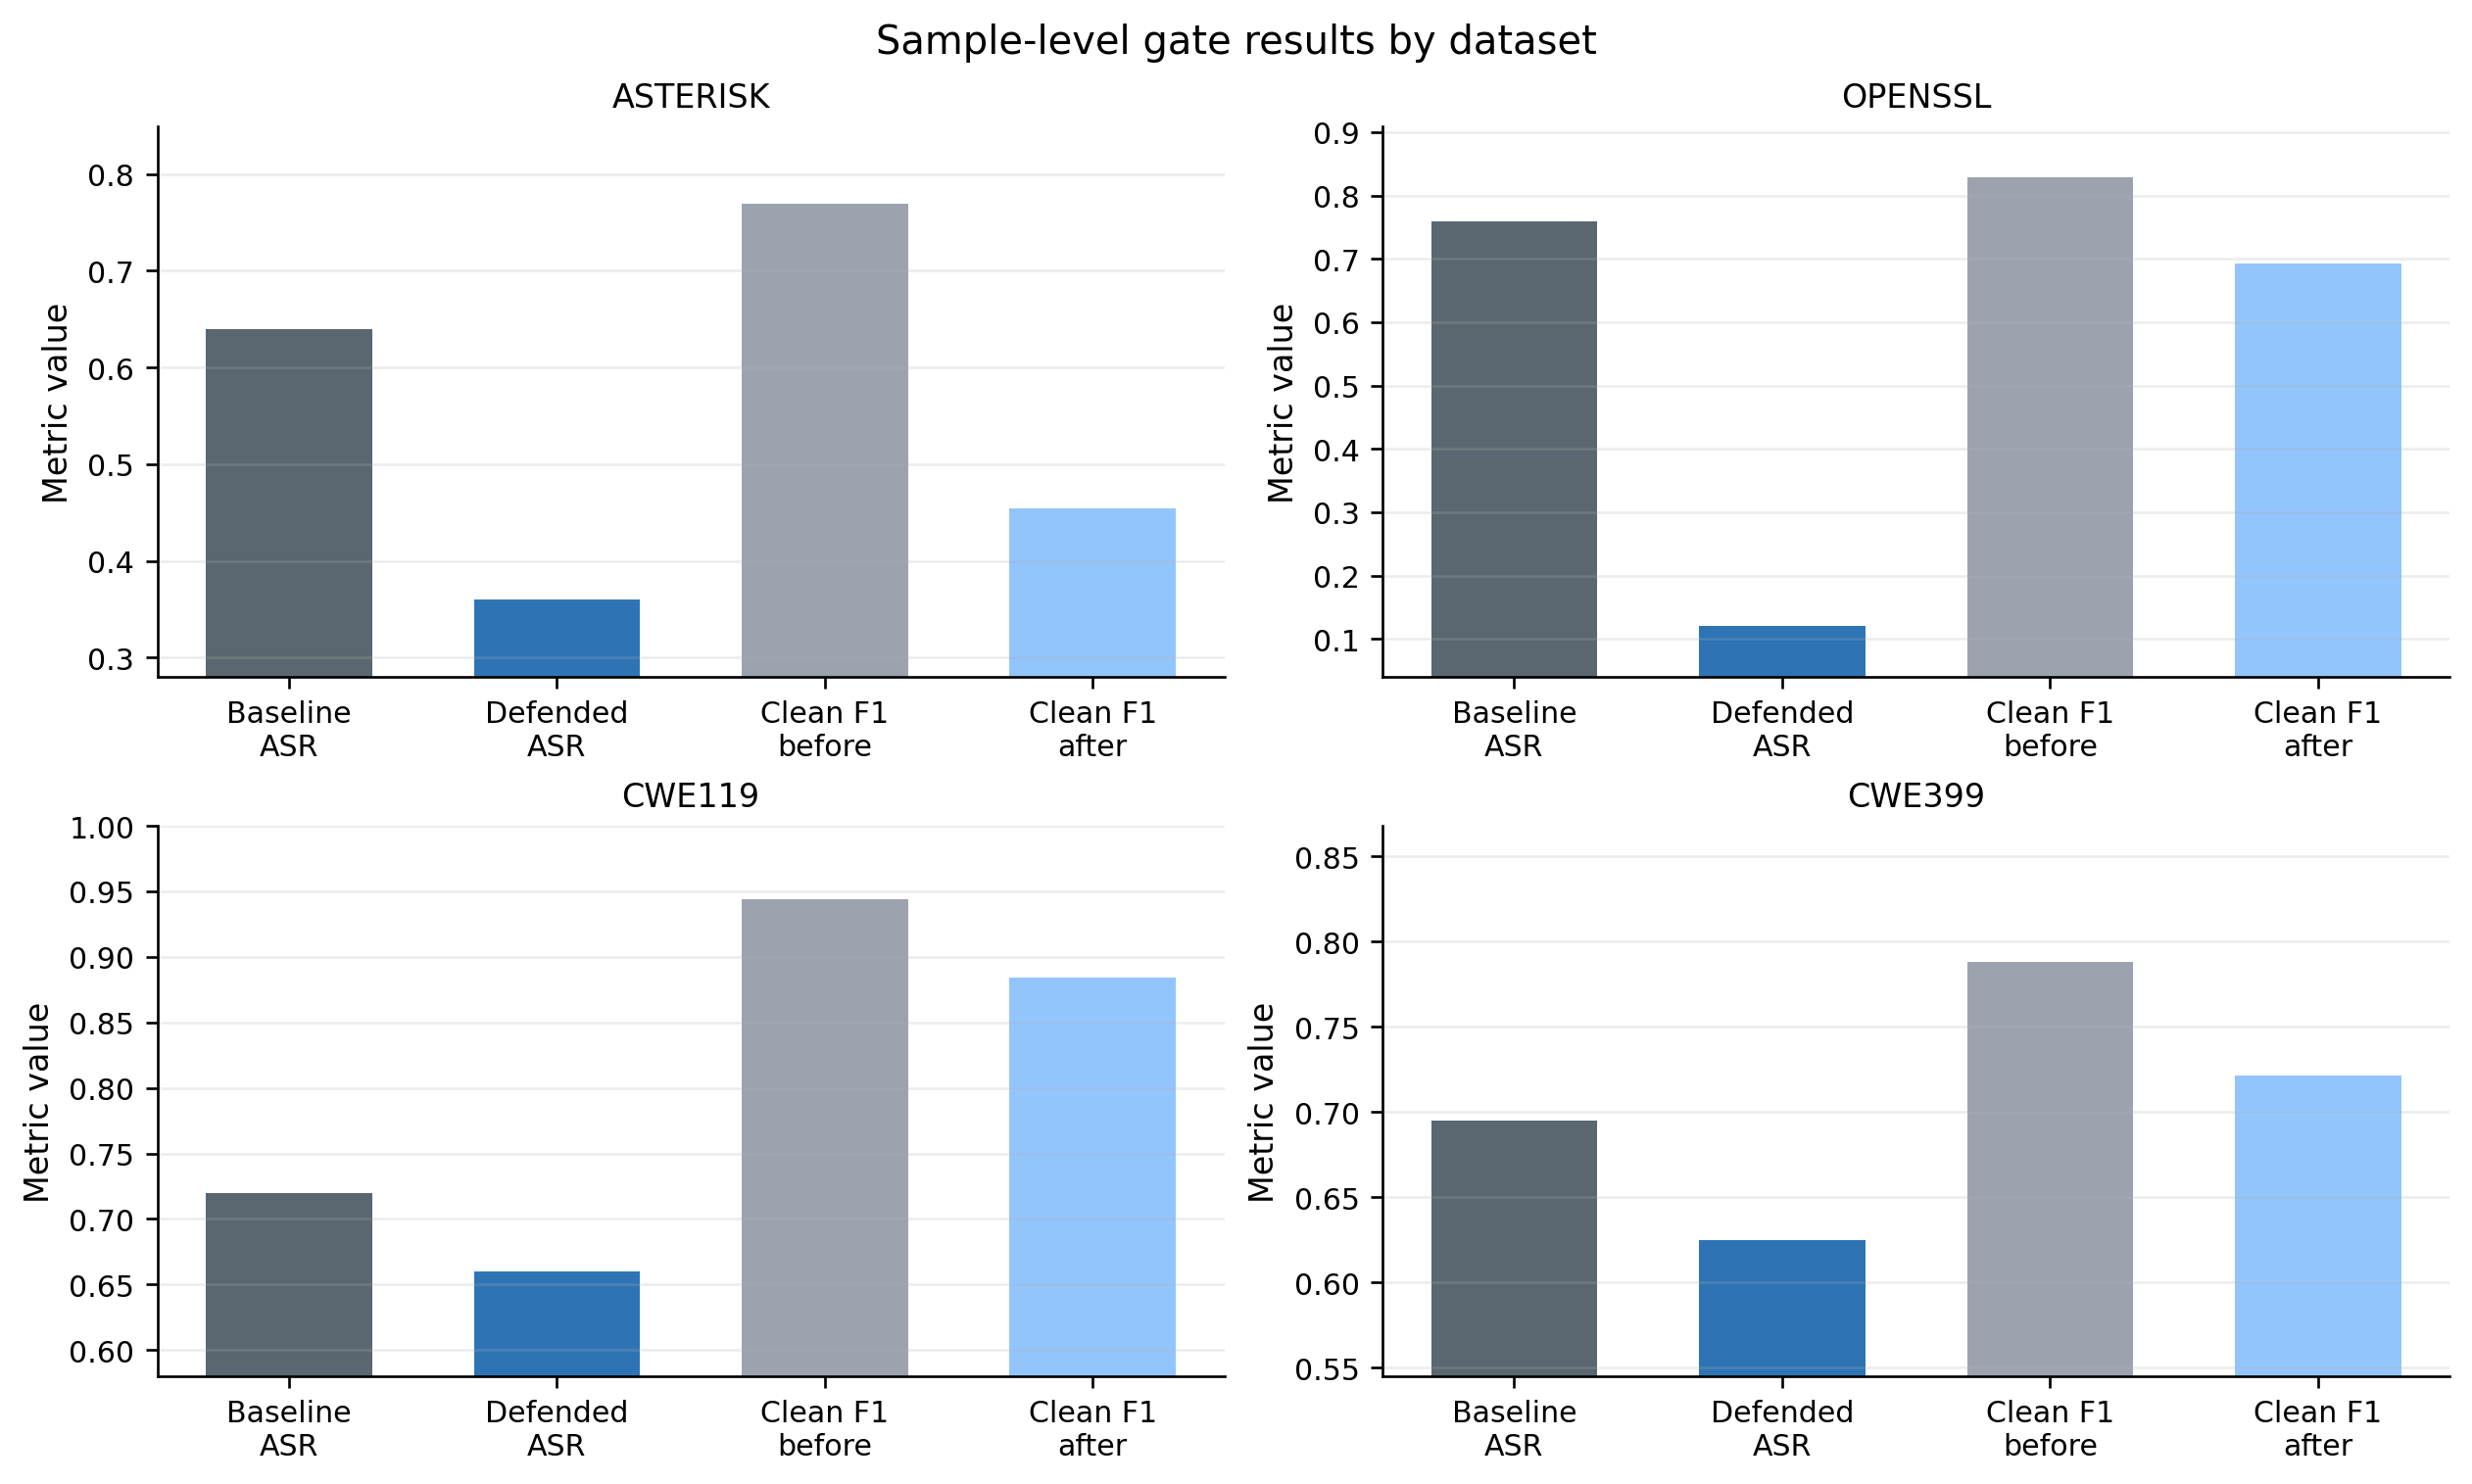
\includegraphics[width=0.88\textwidth]{../figures_submission/sample_gate_results_en.png}
\caption{Sample-level gate results by dataset. Each panel uses an independently scaled y-axis and reports raw \asrshort{}, hard-override \asrshort{}, Clean F1 before hard override, and Clean F1 after hard override. Hard override is an upper-bound diagnostic for the detection signal, not a deployment recommendation.}
  \label{fig:samplegate}
\end{figure*}

\begin{table*}[!t]
\centering
\caption{Descriptive aggregate-count uncertainty checks for the sample-level gate.}
\label{tab:gate-stats}
\resizebox{\textwidth}{!}{%
\begin{tabular}{lrrrrrrr}
\toprule
Dataset & ADV $n$ & Raw bypass & Hard-override bypass & Bypass-rate change (abs.) & Bootstrap 95\% CI & Fisher $p$ & Odds Ratio (95\% CI) \\
\midrule
\dataset{ASTERISK} & 50 & 32 & 18 & 0.280 & [0.100, 0.460] & 0.009 & 3.16 [1.32, 7.56] \\
\dataset{OPENSSL} & 50 & 38 & 6 & 0.640 & [0.480, 0.780] & $8.14{\times}10^{-11}$ & 23.2 [7.2, 80.1] \\
\dataset{CWE119} & 200 & 144 & 132 & 0.060 & [-0.030, 0.150] & 0.234 & N/A \\
\dataset{CWE399} & 200 & 139 & 125 & 0.070 & [-0.025, 0.160] & 0.170 & N/A \\
\bottomrule
\end{tabular}}
\vspace{2pt}
\par\footnotesize\textbf{Note.} These are descriptive aggregate-count uncertainty checks. Fisher tests are interpreted as aggregate-count, distribution-level evidence rather than paired per-sample tests. McNemar tests and paired bootstrap tests require complete per-sample prediction logs and remain future work.
\end{table*}

The aggregate-count checks reinforce the same boundary rather than adding a separate claim. Within the available $n=50$ \dataset{OPENSSL} sample, bypasses fall from 38/50 to 6/50, with Fisher $p=8.14{\times}10^{-11}$ and bootstrap 95\% CI [0.480, 0.780]. \dataset{ASTERISK} is also supported at the aggregate-count level, with a change from 32/50 to 18/50. The smaller mixed-source changes on \dataset{CWE119} and \dataset{CWE399} are not supported by these checks. These aggregate-count checks describe observed distribution-level changes rather than paired per-sample causal claims.

We also report an ablation-style feature-family contribution analysis at the end of RQ1. Table~\ref{tab:gateablation} gives the normalized contribution of four representative feature families tied to EaTVul-style insertion traces. The analysis retrains the leave-one-dataset-out gate and normalizes random-forest importance within these families. As shown in Table~\ref{tab:gateablation}, unseen tokens contribute the largest share, followed by AST-structure features, bigram NLL, and rare-token ratio. These values explain why single-project datasets are easier to defend: unseen-token and structural deviations remain sharper when the clean background distribution is project-coherent.

\begin{table*}[tbp]
\centering
\caption{RQ1: Gate feature-family contribution. Percentages are normalized within the four selected families.}
\label{tab:gateablation}
\begin{tabular}{lrrrr}
\toprule
Split & Rare token & Unseen token & Bigram NLL & AST structure \\
\midrule
LODO average & 11.5\% & 52.9\% & 14.5\% & 21.1\% \\
\bottomrule
\end{tabular}
\vspace{2pt}
\par\footnotesize\textbf{Note.} LODO means leave-one-dataset-out. The contribution percentages are produced by the artifact's feature-importance export script and aggregate summary table. These values do not change the ASR/Clean F1 results in Table~\ref{tab:samplegate}. Feature contributions are normalized to sum to 100\% across the four selected families.
\end{table*}

These rows support detection and quarantine under project-coherent settings, but they do not establish reliable automatic sanitization or broad mixed-source transfer. Whole-sample detection can aggregate rare-token, unseen-token, bigram, and structure-distribution shifts without identifying the exact inserted span.

The gate's strongest feature families match the mechanics of EaTVul-style insertion. Rare-token and unseen-token features fire when inserted snippets introduce identifiers, literals, calls, or library names that are weakly represented in the target project's clean background. Bigram negative log likelihood captures the join between native code and the inserted snippet: even if each token is individually plausible, their local adjacency can be unusual under the clean AST-token language model. AST-structure features capture the fact that inserted snippets often add declarations, control constructs, leaf-node runs, or structural-marker density that changes the whole function's syntax profile. The gate therefore does not merely patch a weakness of the TF-IDF logistic-regression target detector. It detects distributional and structural side effects of adding new code to an existing vulnerable function. This also explains why the signal is strongest on single-project datasets, where the clean coding style is coherent, and weaker on mixed-source datasets, where ordinary clean samples already cover a broader token and structure distribution.

\subsection{RQ2: Comparison with Anomaly-detection Baselines}
Table~\ref{tab:anomaly-baselines} compares the supervised \gate{} with four classic anomaly detectors under the same 10\% clean FPR calibration and the same hard-override diagnostic protocol. The comparison shows that insertion traces are not always global clean-distribution outliers. Within the controlled project-coherent samples, the supervised gate changes the hard-override \asrshort{} by 0.640 on \dataset{OPENSSL}, whereas each unsupervised baseline changes it by only 0.020. On \dataset{ASTERISK}, the best unsupervised change is 0.100, compared with 0.280 for the gate. These rows indicate that attack-versus-clean contrast contributes information that generic outlier scoring misses.

\begin{table*}[tbp]
\centering
\caption{RQ2: Gate versus classic anomaly-detection baselines under the same clean FPR calibration.}
\label{tab:anomaly-baselines}
\resizebox{\textwidth}{!}{%
\renewcommand{\arraystretch}{1.05}%
\begin{tabular}{lrrrrrr}
\toprule
\multirow{2}{*}{Method} & \multicolumn{3}{c}{\dataset{OPENSSL}} & \multicolumn{3}{c}{\dataset{ASTERISK}} \\
\cmidrule(lr){2-4}\cmidrule(lr){5-7}
 & Hard-override ASR & ASR change (abs.) & ADV recall & Hard-override ASR & ASR change (abs.) & ADV recall \\
\midrule
Supervised Gate & 0.120 & 0.640 & 0.740 & 0.360 & 0.280 & 0.280 \\
Isolation Forest & 0.740 & 0.020 & 0.080 & 0.540 & 0.100 & 0.120 \\
One-Class SVM & 0.740 & 0.020 & 0.060 & 0.580 & 0.060 & 0.100 \\
Local Outlier Factor & 0.740 & 0.020 & 0.060 & 0.560 & 0.080 & 0.120 \\
Mahalanobis & 0.740 & 0.020 & 0.060 & 0.600 & 0.040 & 0.160 \\
\bottomrule
\end{tabular}}
\vspace{2pt}
\par\footnotesize\textbf{Note.} Clean non-vulnerable FPR is 0.100--0.104 across methods after target-dataset calibration.
\end{table*}

The baseline comparison clarifies what kind of detection capability is available. The artifact contains weak distributional and structural traces of insertion, but those traces are not equivalent to ordinary outliers. Generic anomaly detectors model global distance from the clean distribution and therefore miss attacks that remain plausible under the target distribution. The supervised gate performs better because it learns fine-grained insertion signatures, including local bigram joins, shifts in structural-token ratios, unusual runs of declarations or control markers, and rare project-specific identifiers. This narrows the claim: AST-token-only detection is feasible when attack-aware calibration is available, but generic anomaly detection alone is not a reliable substitute.

RQ2 therefore separates the detection boundary from a generic anomaly-detection boundary. Effective screening under project-coherent settings requires insertion-specific evidence, while generic unsupervised filtering leaves most silent bypasses intact.

\subsection{RQ3: Bounded Model-coverage Sanity Check}
Table~\ref{tab:neural-targets} reports the bounded model-coverage sanity check on \dataset{OPENSSL} and \dataset{ASTERISK}. The question is whether bypassed samples under a neural target still carry AST-token-level insertion traces that the same detection signal can screen. CodeBERT-base is the primary sanity-check row. This check does not change the paper into a broad neural-detector evaluation; within the available $n=50$ project-coherent attack sets, it tests only whether the gate signal remains visible outside the linear TF-IDF target setting. BiLSTM-attention is retained in Appendix B, Table~\ref{tab:bilstm-appendix}, as an additional neural reference, not as central evidence.

\begin{table*}[tbp]
\centering
\caption{RQ3: Bounded model-coverage sanity check for gate screening. CodeBERT-base is the primary sanity-check row.}
\label{tab:neural-targets}
\resizebox{\textwidth}{!}{%
\renewcommand{\arraystretch}{1.05}%
\begin{tabular}{L{1.7cm}L{3.1cm}R{1.1cm}R{1.2cm}R{1.2cm}R{1.4cm}R{2.4cm}}
\toprule
Dataset & Target detector & Train $n$ & Clean F1 & ADV ASR & Bypassed & Gate recall on bypasses \\
\midrule
\dataset{OPENSSL} & CodeBERT-base & 160 & 0.436 & 0.820 & 41/50 & 0.780 \\
\dataset{ASTERISK} & CodeBERT-base & 150 & 0.260 & 0.480 & 24/50 & 0.542 \\
\bottomrule
\end{tabular}}
\vspace{2pt}
\par\footnotesize\textbf{Note.} The gate is unchanged and calibrated at 10\% clean FPR. These rows test whether the detection signal is visible beyond the TF-IDF target detector; they are not accuracy-optimized vulnerability-detector benchmarks.
\end{table*}

The CodeBERT-base rows provide limited evidence that the gate signal can remain visible under a neural target in the evaluated project-coherent rows. On \dataset{OPENSSL}, CodeBERT-base leaves 41 adversarial samples as benign bypasses, and the unchanged gate screens 0.780 of those bypasses. On \dataset{ASTERISK}, it leaves 24 bypasses and the gate screens 0.542. The low Clean F1 values should not be read as optimized CodeBERT vulnerability-detection performance. They reflect the bounded sanity-check setup: only small balanced training subsets are available, fine-tuning is limited to one epoch, and serialized AST-token sequences differ from the natural-language/code distributions used in CodeBERT pretraining. These rows do not support a claim about neural-detector accuracy across architectures.

RQ3 suggests, within this bounded sanity-check setting, that the gate signal is not purely an artifact of the linear TF-IDF target. The result remains limited to the evaluated project-coherent rows and should not be read as a broad neural-detector evaluation.

\subsection{RQ4: Fixed-window Diagnostic Deletion Test}
Table~\ref{tab:sanitization-summary} summarizes the two diagnostic deletion tests. Fixed-window deletion can remove suspicious regions, but token-window localization lacks the source boundary needed for recovery. Within the controlled \dataset{OPENSSL} row, the fixed-window method modifies many adversarial samples, but the post-deletion ASR decrease is only 0.060. On \dataset{CWE119} and \dataset{CWE399}, the same strategy produces no post-deletion ASR change. These results show that suspicious-token deletion is not equivalent to removing the injected source code.

\begin{table*}[tbp]
\centering
\caption{Diagnostic deletion boundary-test summary. These deletion tests are not deployable sanitizers and do not verify source-level, semantics-preserving repair; detailed token-modification proxy metrics are reported separately in Table~\ref{tab:sanitization-details}.}
\label{tab:sanitization-summary}
\resizebox{\textwidth}{!}{%
\renewcommand{\arraystretch}{1.05}%
\begin{tabular}{llrrrrr}
\toprule
Dataset & Method & Clean F1 before & Clean F1 after & Raw ASR & Post-deletion ASR & ASR change (abs.) \\
\midrule
\dataset{ASTERISK} & Fixed window & 0.769 & 0.274 & 0.640 & 0.600 & 0.040 \\
\dataset{OPENSSL} & Fixed window & 0.829 & 0.819 & 0.760 & 0.700 & 0.060 \\
\dataset{CWE119} & Fixed window & 0.944 & 0.943 & 0.720 & 0.720 & 0.000 \\
\dataset{CWE399} & Fixed window & 0.788 & 0.788 & 0.695 & 0.695 & 0.000 \\
\dataset{ASTERISK} & AST-token component & 0.769 & 0.265 & 0.640 & 0.600 & 0.040 \\
\dataset{OPENSSL} & AST-token component & 0.829 & 0.829 & 0.760 & 0.760 & 0.000 \\
\dataset{CWE119} & AST-token component & 0.944 & 0.941 & 0.720 & 0.720 & 0.000 \\
\dataset{CWE399} & AST-token component & 0.788 & 0.780 & 0.695 & 0.695 & 0.000 \\
\bottomrule
\end{tabular}}
\vspace{2pt}
\par\footnotesize\textbf{Note.} Both methods are diagnostic boundary tests. Token deletion is not verified source-level, semantics-preserving sanitization and does not validate exact inserted-span deletion. The fixed-window row uses clean window FPR 0.01, 1536-token windows, 768-token stride, at most two spans, benign-only gating, no sample-level gate, and $\delta_w=0.005$. The AST-token component row uses clean component FPR 0.01, maximum cluster size 3, maximum one selected span, benign-only gating, no sample-level gate, and $\delta_c=0.001$.
\end{table*}

The strongest modification row illustrates the information gap. On \dataset{OPENSSL}, the fixed-window deletion test modifies 0.760 of adversarial samples and removes 0.434 of adversarial tokens on average, while \cleanf{} changes only from 0.829 to 0.819. Yet the post-deletion ASR decrease is limited, from 0.760 to 0.700. This mismatch means the artifact can identify suspicious regions without identifying the correct deletion boundary. A fixed window can straddle native code and the inserted snippet, delete vulnerability-evidence tokens needed for recovery, or miss the small inserted fragment that caused the benign prediction. On \dataset{ASTERISK}, the limited post-deletion ASR decrease is accompanied by a severe \cleanf{} drop, confirming that token-only deletion can damage utility.

RQ4 shows that the evaluated fixed-window method does not achieve reliable sanitization from suspicious-token localization alone. Without source spans and insertion boundaries, the defensible action remains quarantine rather than automatic deletion.

\subsection{RQ5: AST-token Component-level Diagnostic Deletion Test}
Table~\ref{tab:sanitization-summary} also reports the AST-token component diagnostic deletion test. Adding token-structure proxies improves interpretability, but it does not overcome the absence of true program structure. The component-level method changes \asrshort{} by 0.040 on \dataset{ASTERISK} and by 0.000 on the other three datasets. Approximate components can make candidate regions more interpretable, but they do not provide the evidence needed to restore vulnerable predictions reliably.

The component results separate interpretability from correctness. On \dataset{OPENSSL}, 0.740 of adversarial samples are modified and \cleanf{} remains 0.829, but residual \asrshort{} stays 0.760. The deletion operation therefore changes tokens without restoring the vulnerable prediction. On \dataset{ASTERISK}, \cleanf{} drops to 0.265, showing that even structure-inspired proxies can remove useful clean evidence. The low removed-token ratios on \dataset{CWE119} and \dataset{CWE399} further indicate that approximate component boundaries do not reliably capture inserted spans. These components are not source spans, CFG regions, or PDG-isolated slices; they can still straddle native and inserted code, remove vulnerability-relevant tokens, or fail to isolate the evasion-relevant snippet.

RQ5 reinforces the diagnostic deletion boundary for the evaluated component method. More structured token units produced only a limited recovery effect in the absence of true source spans, CFGs, and PDGs.

These negative diagnostic deletion results should not be interpreted merely as implementation failures. Rather, they show that serialized AST-token evidence lacks the localization and semantic-dependency information required for reliable automatic sanitization. Under the evaluated public-artifact setting, quarantine is therefore a more defensible endpoint than automatic sanitization.

A future source-aware subset should add compiler-validated samples, exact source-to-token mappings, true inserted spans, deletion precision/recall/IoU, compilation-success checks, and a semantic-preservation proxy. Such a subset would allow deletion precision to be measured directly instead of inferred from token-removal ratios. It is not part of the present artifact.

\subsection{RQ6: Quarantine and F1-constrained Calibration}
Table~\ref{tab:quarantine} reports quarantine with a clean review-routing budget of 0.10, and Table~\ref{tab:f1constrained} reports F1-constrained override with maximum \cleanf{} drop 0.030. Quarantine converts suspicion into review rather than unsupported repair. It keeps suspicious benign predictions from passing silently, while F1-constrained override protects clean utility by accepting less security gain.

\begin{table}[tbp]
\centering
\caption{RQ6: Quarantine policy with clean review-routing budget 0.10. Residual silent-bypass rate counts only adversarial samples that still pass automatically as benign; Quar. is the clean quarantine rate.}
\label{tab:quarantine}
\scriptsize
\setlength{\tabcolsep}{2pt}
\begin{tabular}{L{1.35cm}R{1.05cm}R{1.05cm}R{2.25cm}R{0.85cm}}
\toprule
Dataset & Clean F1 & Base ASR & Residual silent-bypass rate & Quar. \\
\midrule
\dataset{ASTERISK} & 0.769 & 0.640 & 0.360 & 0.093 \\
\dataset{OPENSSL} & 0.829 & 0.760 & 0.120 & 0.085 \\
\dataset{CWE119} & 0.944 & 0.720 & 0.650 & 0.059 \\
\dataset{CWE399} & 0.788 & 0.695 & 0.625 & 0.082 \\
\bottomrule
\end{tabular}
\vspace{2pt}
\par\footnotesize\textbf{Note.} Quarantined adversarial samples are counted as review-routed silent bypasses, not as automatic label corrections. The deployment cost is review load rather than clean-label relabeling.
\end{table}

\begin{table}[tbp]
\centering
\caption{RQ6: F1-constrained hard override with maximum Clean F1 drop 0.030. This is a utility-constrained diagnostic override policy, not quarantine.}
\label{tab:f1constrained}
\scriptsize
\setlength{\tabcolsep}{2pt}
\renewcommand{\arraystretch}{1.05}
\begin{tabular}{L{1.25cm}R{0.78cm}R{0.78cm}R{0.72cm}R{0.76cm}R{0.76cm}R{0.90cm}}
\toprule
Dataset & F1 before & F1 after & F1 drop & Raw ASR & H.O. ASR & ASR change (abs.) \\
\midrule
\dataset{ASTERISK} & 0.769 & 0.741 & 0.028 & 0.640 & 0.640 & 0.000 \\
\dataset{OPENSSL} & 0.829 & 0.800 & 0.029 & 0.760 & 0.520 & 0.240 \\
\dataset{CWE119} & 0.944 & 0.940 & 0.003 & 0.720 & 0.710 & 0.010 \\
\dataset{CWE399} & 0.788 & 0.788 & 0.000 & 0.695 & 0.695 & 0.000 \\
\bottomrule
\end{tabular}
\vspace{2pt}
\par\footnotesize\textbf{Note.} H.O. ASR denotes hard-override ASR. The threshold is chosen under a maximum Clean F1 drop of 0.030; tighter utility constraints leave more adversarial samples accepted automatically.
\end{table}

Quarantine preserves the security effect of detection without claiming to correct the label or repair the code. On \dataset{OPENSSL} and \dataset{ASTERISK}, the residual silent-bypass rates are 0.120 and 0.360, with clean quarantine rates of 0.085 and 0.093. F1-constrained calibration shows the opposite tradeoff. On \dataset{OPENSSL}, hard override changes \asrshort{} by 0.240 while keeping F1 drop at 0.029, but on the other datasets the utility constraint leaves little or no protection. The practical boundary is that AST-token-only evidence can justify review routing, but not automatic relabeling or sanitization as the default response.

\begin{figure*}[tbp]
  \centering
  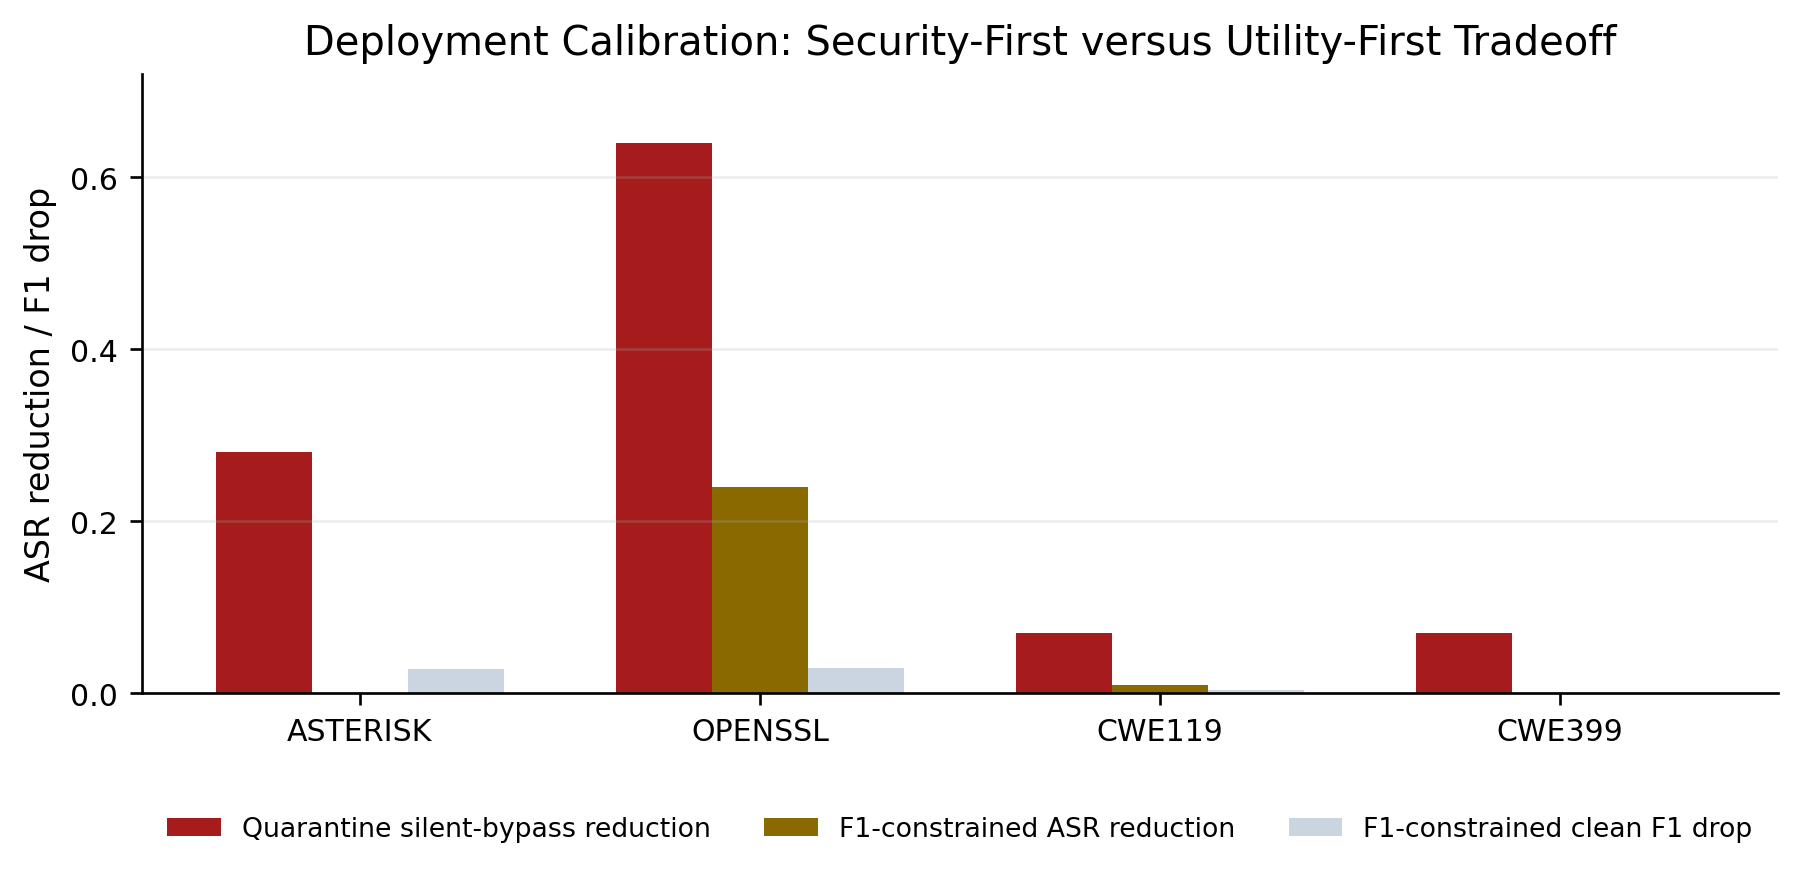
\includegraphics[width=0.72\textwidth]{../figures_submission/deployment_tradeoff_en.png}
\caption{Deployment calibration tradeoff. Security-first quarantine uses review routing to prevent suspicious benign decisions from automatic acceptance; quarantine is review routing, not prediction correction. Utility-first F1-constrained calibration preserves clean utility but leaves more adversarial samples to pass automatically.}
  \label{fig:deployment}
\end{figure*}

RQ6 identifies quarantine as the most defensible deployment mode for AST-token-only defense. F1-constrained override is useful only when clean utility dominates and the remaining silent-bypass risk is acceptable.

\subsection{Supplementary Source-text Stress Checks}
The source-text extension is retained as an artifact interface and diagnostic stress-check harness. It broadens inspection from the public AST-token artifact to source-text project splits, but the generated snippets are not compiler-validated and are not used as main-claim evidence.

Appendix~A summarizes the source-text diagnostic material that should be supplied separately as supplementary rows. The larger source-text rows are mixed rather than uniformly positive, and the small-case rows remain underpowered. These rows identify where future source-aware experiments should add compiler validation, source spans, and per-sample logs. They do not change the main paper's evidentiary basis, which is the public AST-token artifact.

\subsection{Integrated Comparison}
Table~\ref{tab:comparison} summarizes the deployable gate/quarantine path, the two diagnostic boundary tests, the numeric anomaly baselines, and adversarial training as a qualitative comparator. The main text keeps the comparison compact; Table~\ref{tab:comparison-full} reports the full comparison with granularity, action, deployable-defense status, policy-specific bypass effect, \cleanf{} cost, interpretability, and limitation.

\begin{table*}[tbp]
\centering
\caption{Integrated comparison summary of the deployable gate/quarantine path, diagnostic boundary tests, deployment policies, and common defense baselines.}
\label{tab:comparison}
\resizebox{\textwidth}{!}{%
\begin{tabular}{L{3.1cm}L{2.0cm}L{4.8cm}L{4.8cm}}
\toprule
Method & Deployable defense? & Main effect & Main limitation \\
\midrule
No defense & N/A / Baseline & Leaves adversarial vulnerable samples to pass silently as benign. & No protection against insertion evasion. \\
Classic anomaly detection & Partial & Provides weak unsupervised filtering under the same clean FPR budget. & Much weaker than insertion-specific gate learning. \\
Adversarial training & Partial & Retrains a target detector on representative attack variants. & Needs generated variants and gives no quarantine or localization path. \\
\Gate{} & Yes, as screening for quarantine & Under project-coherent settings, detects many bypasses; hard override changes \asrshort{} by 0.640 on \dataset{OPENSSL} and 0.280 on \dataset{ASTERISK}. & Depends on project-coherent calibration; weak transfer on mixed-source datasets. \\
\Windowdef{} & No & Removes suspicious token windows in the Section~\ref{sec:reliable-sanitization} diagnostic boundary test. & Windows may cut native syntax and miss true snippets. \\
\Componentdef{} & No & Improves interpretability over raw windows with approximate AST-token regions. & Components are not true AST/CFG/PDG regions. \\
Quarantine & Yes & Preserves gate security gains while routing suspicious benign decisions to review. & Requires human or secondary review capacity. \\
F1-constrained gate & Partial & Bounds clean-utility loss while retaining some protection. & Tight utility constraints can leave attacks to pass automatically. \\
\bottomrule
\end{tabular}}
\vspace{2pt}
\par\footnotesize\textbf{Note.} Reported \asrshort{} changes are policy-specific: gate rows use hard-override diagnostics, while quarantine rows use residual silent-bypass rates. Full details appear in Table~\ref{tab:comparison-full}.
\end{table*}

\subsection{Failure Case Analysis}
The available artifacts do not provide complete paired prediction logs, true inserted spans, or source diffs for every defense layer. We therefore report representative failure modes grounded in aggregate behavior rather than sample-specific forensic cases.

\textbf{Case 1: mixed-source gate failure.} On \dataset{CWE119} and \dataset{CWE399}, adversarial recall is only 0.060 and 0.070 under the same 10\% clean-FPR calibration. These datasets combine broader clean distributions, so insertion traces overlap more with ordinary clean variation. The rare-token, unseen-token, bigram-NLL, and structural signals that separate attacks in a project-coherent setting become less distinctive when the clean background already contains many projects, coding styles, and vulnerability contexts. The failure mode is therefore not that the gate lacks any useful signal; rather, the calibrated signal is too weak to quarantine most mixed-source bypasses without increasing clean review load. This corresponds to the mixed-source transfer boundary identified in RQ1 and RQ2.

\textbf{Case 2: deletion without recovery.} The fixed-window deletion test modifies 0.760 of adversarial \dataset{OPENSSL} samples and removes 0.434 of adversarial tokens on average, yet \asrshort{} falls only from 0.760 to 0.700. The component-level deletion test shows the same pattern more sharply: it modifies 0.740 of adversarial \dataset{OPENSSL} samples while residual \asrshort{} remains 0.760. These aggregate rows indicate a concrete failure mode: the method can remove tokens that look suspicious without removing the source-level insertion in a way that restores the vulnerable prediction. Because the deletion unit is an arbitrary window or approximate token component, it can cut across native and inserted code, remove vulnerability evidence, or leave the evasion-relevant context intact. Without source spans, CFG reachability, or dependence information, the method cannot distinguish these outcomes. This is the recovery failure emphasized by RQ4 and RQ5.

\textbf{Case 3: clean-utility damage.} On \dataset{ASTERISK}, both diagnostic deletion tests change \asrshort{} by only 0.040 while \cleanf{} drops from 0.769 to 0.274 for fixed windows and to 0.265 for component-level deletion. This is the opposite of reliable sanitization: the deletion rule changes clean behavior far more than it recovers vulnerable predictions. The case illustrates why suspicious-token localization should not be treated as verified source-level sanitization under AST-token-only evidence. This reinforces the preservation criterion in the diagnostic boundary tests.

\section{Discussion}
\subsection{Supported Capabilities}
The evaluated evidence supports sample-level suspicion scoring and quarantine under project-coherent AST-token-only settings. This capability is valuable because it does not require the defense to know where the injected code begins or ends. It only requires enough distributional and structural evidence to decide that a benign prediction should not be accepted automatically. The strongest results occur when the clean background is project-coherent, and the bounded CodeBERT-base sanity check provides limited evidence that the same gate signal remains visible under a neural target in those rows. The weak \dataset{CWE119} and \dataset{CWE399} rows show that this support does not transfer reliably to mixed-source datasets.

Quarantine is the most stable deployment form of this capability. For a single-project internal detection platform, the recommended deployment is a sample-level detection gate followed by human review or secondary source-aware analysis; the project-coherent rows suggest that this workflow can substantially reduce silent bypasses at a review load near the calibrated budget. For a cross-project public detection service, the mixed-source rows are a warning: pure AST-token gating is too weak to serve as the primary mitigation, and should be combined with richer context, project-aware calibration, or conservative review policies. In both settings, quarantine treats the gate output as a review-routing signal rather than a corrected vulnerability label.

\subsection{Remaining Insufficient Capabilities}
The current evaluation did not validate reliable automatic sanitization. This limitation reflects both the information available in the artifact and the design of the evaluated token-only methods. The artifact lacks source spans, exact insertion boundaries, parser-validated edit units, CFG reachability, and PDG dependence information. The evaluated methods use fixed windows and approximate components that cannot compensate for these omissions.

The diagnostic deletion experiments therefore mark the evidentiary gap defined in Section~\ref{sec:reliable-sanitization}. Fixed windows and approximate AST-token components can remove suspicious token regions, but they cannot establish that the removed region corresponds to injected source code or that the remaining program representation still preserves the vulnerability signal. This conclusion applies only to the two representative token-only deletion strategies evaluated here. Stronger sequence-labeling methods, large-language-model-guided token localization, or richer token-structure approximations may improve recovery, but without source code they still cannot verify syntax correctness, semantic preservation, or dependence isolation. The experiments therefore motivate source-aware evidence for reliable automatic sanitization without formally excluding every possible token-only method. In this sense, the failure of token-only deletion is a boundary finding: detection can rely on distributional traces, whereas sanitization requires localization and dependency information that the serialized public artifact does not preserve.

\subsection{Implications for Future Systems}
The short-term deployment path is an AST-token detection plus quarantine workflow. Such a system can score benign predictions for insertion-like evidence and route suspicious samples to human or secondary review. This operating mode fits settings where the defender has public artifacts but not complete source-code authority. It preserves the value of AST-token evidence while avoiding unsupported deletion. A short-term research goal is to construct larger project-coherent AST-token datasets with true insertion boundaries and to evaluate stronger token-level detection methods under the same leakage-free protocol.

The mid-term path is to quantify the information-performance curve for sanitization. Source line numbers, statement boundaries, CFG reachability, and PDG dependence information should be added incrementally to measure which evidence dimension produces which recovery and preservation gain. The long-term path is source-aware automatic sanitization, potentially assisted by large language models for token-level semantic validation. A future system will likely need source spans, exact insertion boundaries, CFGs, and PDGs in addition to the public artifact. Source spans can align suspicious tokens with statements or subtrees. CFGs can test reachability and guarded branches. PDGs can test whether a candidate deletion is isolated from vulnerability-relevant data and control dependencies. Model feedback can still be useful, but it should confirm source-aware deletion candidates rather than define the deletion boundary from tokens alone. The broader design lesson is to combine public artifacts with program-context evidence when the goal is reliable automatic sanitization, while leaving room for future work on stronger token-only approximations.

This boundary analysis motivates larger compiler-validated adversarial datasets with exact source-to-token mappings for future evaluations.

\section{Limitations and Threats to Validity}
\subsection{Dataset and Statistical Scope}
The main numerical evidence is bounded by the available public EaTVul-style AST-token artifacts. \dataset{ASTERISK} and \dataset{OPENSSL} contain 50 adversarial test samples each, which limits statistical power and makes confidence intervals sensitive to a small number of prediction changes. \dataset{CWE119} and \dataset{CWE399} are larger mixed-source stress settings, but their broader clean distributions weaken the same gate signal. Fisher exact tests and bootstrap intervals are therefore used as descriptive aggregate-count, distribution-level checks rather than paired per-sample causal tests. Complete paired logs are not available for all defense layers, so future artifact versions should add per-sample prediction logs, McNemar tests for paired bypass/non-bypass changes, paired bootstrap confidence intervals for \asrshort{} or residual silent-bypass reductions, multi-seed means and standard deviations, and exact confidence intervals for small-$n$ rows such as \dataset{OPENSSL} and \dataset{ASTERISK}. The numerical changes should be read as evidence for a capability boundary, not as broad deployment claims.

\subsection{Model and Attack Coverage}
The main experiments use a TF-IDF plus logistic-regression target detector as a controlled and auditable carrier for the public AST-token artifact. RQ3 adds CodeBERT-base only as a bounded model-coverage sanity check. The BiLSTM-attention and LineVul rows are supplementary reference or stress-check rows, not main evidence. The attack coverage is also bounded: the evaluation studies EaTVul-style insertion evasion, where the original vulnerability remains and added code shifts the detector toward a benign prediction. It does not cover identifier renaming, statement reordering, expression substitution, formatting changes, or other evasion families. The attacker is non-adaptive with respect to the gate. Adaptive mimicry attacks may reduce rare-token, unseen-token, and bigram-NLL signals, so they remain future work.

\subsection{Observation Constraint and Construct Validity}
The central construct is the observation-constrained public-artifact setting. The defender observes serialized AST-token sequences and detector outputs, but not source spans, source diffs, exact insertion boundaries, CFGs, or PDGs. This constraint limits what the evaluation can validate. The \textit{ADV removed ratio} is a token-removal proxy, not insertion-span recall. Quarantine is review routing, not source correction. Reliable sanitization follows the recovery, preservation, and precision criteria defined in Section~\ref{sec:reliable-sanitization}, which are stricter than token deletion or vulnerable-probability gain. The evaluated deletion tests therefore probe a boundary; they do not verify source-level, semantics-preserving sanitization.

\subsection{Serialization and Deployment Scope}
The results depend on the specific AST-token serialization used in the public artifact. Other tree linearizations, marker vocabularies, or tokenization conventions could change local bigram statistics, structural-marker density, and gate calibration. The deployment interpretation also depends on review capacity. Quarantine can reduce silent bypasses only when suspicious samples can be reviewed or sent to a stronger source-aware analysis. In mixed-source settings, where gate recall is weaker and clean review load can still be nontrivial, the cost-benefit ratio of quarantine may deteriorate. Future evaluations should test multiple serializations, project-aware calibration strategies, and review-capacity constraints.

\section{Reproducibility and Artifact Availability}
The review artifact is maintained at \url{https://github.com/xk-05/eatvul-jisa-artifact}. The public repository contains the manuscript source, bibliography, figures, experiment/table scripts, configurations, aggregate result tables, and selected CSV/JSON/JSONL outputs used for the reported rows. The main evaluation uses four EaTVul-style AST-token datasets: \dataset{ASTERISK}, \dataset{OPENSSL}, \dataset{CWE119}, and \dataset{CWE399}. Because the redistribution terms for the external AST-token split files are not confirmed in this package, the public Git repository does not redistribute those split files. Full reruns and dataset-size checks require users to prepare the clean-train, clean-test, and adversarial-test splits locally under the paths documented in the artifact.

The artifact includes the experiment configuration for the \gate{}, anomaly baselines, diagnostic deletion boundary tests, deployment policies, and extension harness, together with trained gate settings, calibrated thresholds, aggregate result tables, and per-sample prediction logs where available.

\paragraph{Artifact checklist.} The current package contains or should retain code, configurations, data splits where available, calibrated thresholds, per-sample prediction logs where available, table-generation scripts, random seeds, environment notes, and aggregate result tables. These objects are sufficient to reproduce the reported aggregate tables and to audit the thresholding and deployment-policy choices, but they are not a complete paired-log release for every defense layer.

Several objects are not available in the current AST-token-only setting: true inserted spans, source diffs, CFGs, PDGs, compiler-validated adaptive snippets, and complete paired prediction logs for all defense layers. The extension harness records generated insertion metadata and validation status for source-text stress checks, but this metadata is not a substitute for true ground-truth insertion diffs or compiler-validated semantics-preserving attacks. The artifact also includes the LineVul Big-Vul extension harness as a supplementary tool for future source-text stress testing; it is not used to support the main claims. These missing objects are not incidental implementation details. They are the evidence needed to validate source-aware deletion and dependence isolation. Their absence is part of the capability boundary claim: whole-sample detection and quarantine can be evaluated from AST-token sequences, while the evaluated token-only sanitization methods did not achieve reliable automatic sanitization without source-aware artifacts.

\section{Ethics and Responsible Use}
This work is defensive. It does not introduce a new attack-generation algorithm or new prompts for producing evasive snippets. The experiments use existing public EaTVul-style adversarial samples and focus on reducing silent false negatives in vulnerability detection. Artifact releases should emphasize defense code, configuration, and evaluation scripts, and should avoid packaging additional attack-generation tools beyond already public resources.

\section{Conclusion}
This paper studied what defensive behavior remains possible when an EaTVul-style evasion defense can observe only serialized AST-token artifacts. Instead of proposing another vulnerability detector, it evaluated three capabilities under that observation constraint: detection, quarantine, and automatic sanitization.

The findings are conditionally asymmetric. Under project-coherent settings, AST-token evidence supports sample-level suspicion scoring and quarantine. The bounded CodeBERT-base sanity check provides limited evidence that this gate signal is not purely an artifact of the linear TF-IDF target in the evaluated project-coherent setting. The weak mixed-source rows show that the detection support transfers poorly outside those settings. The same evidence did not support reliable automatic sanitization with the evaluated fixed-window and approximate AST-token-component methods; this negative result identifies missing program-analysis information but does not formally exclude stronger token-only approaches.

Overall, our results show that serialized AST-token evidence preserves enough distributional and structural traces to support suspicious benign prediction detection and quarantine. However, the same evidence does not preserve the source-level boundaries and semantic dependencies required for reliable automatic sanitization. Under current public EaTVul artifacts, quarantine is therefore a defensible endpoint, whereas reliable automatic sanitization should require richer source-level and program-analysis representations.

\section*{CRediT authorship contribution statement}
Kang Xie: Conceptualization, Methodology, Software, Validation, Formal analysis, Investigation, Data curation, Writing - original draft, Writing - review \& editing, Visualization.

\section*{Declaration of competing interest}
The author declares that there are no known competing financial interests or personal relationships that could have appeared to influence the work reported in this paper.

\section*{Funding}
This research did not receive any specific grant from funding agencies in the public, commercial, or not-for-profit sectors.

\section*{Declaration of generative AI and AI-assisted technologies in the manuscript preparation process}
During preparation of this work, the author used OpenAI Codex to assist with language polishing, consistency checks between the manuscript and artifact repository, and repository-quality checks. The author reviewed and edited the generated suggestions and takes full responsibility for the content of the published article.

\section*{Data availability}
The experiments use EaTVul-style AST-token artifacts. The public repository contains manuscript sources, implementation scripts, configurations, calibrated thresholds where available, figure/table-generation scripts, aggregate result tables, and selected per-sample prediction logs. The external AST-token split files are not redistributed through public Git tracking because their upstream redistribution terms are not confirmed in this package; preparation paths, expected counts, and checksum notes are documented in the artifact. True inserted spans, source diffs, CFGs, PDGs, compiler-validated adaptive snippets, and complete paired prediction logs for all defense layers are unavailable in the current public AST-token-only setting.

\FloatBarrier
\clearpage
\bgroup
\small
\bibliographystyle{IEEEtran}
\bibliography{references}
\egroup

\clearpage
\onecolumn
\noindent\textit{Appendix figures and tables continue the main-text numbering.}
\par\vspace{4pt}
\section*{Appendix A: Supplementary Source-text Diagnostic Summary}
\noindent These rows are supplementary diagnostics and are not used as evidence for the main claims. The main evidentiary basis remains the public AST-token artifact evaluated in RQ1--RQ6. The source-text stress harness, LineVul checkpoint rows, and non-compiler-validated generated-snippet rows are retained only to document future source-aware evaluation directions. They are not compiler-validated, do not provide true inserted-span ground truth, and do not support claims about deployable repair or reliable automatic sanitization.

\begin{table}[!htbp]
\centering
\caption{Supplementary diagnostic material excluded from the main claims. These rows are supplementary diagnostics and are not used as evidence for the main claims.}
\label{tab:adaptive-plan}
\small
\renewcommand{\arraystretch}{1.08}%
\begin{tabular}{L{3.1cm}L{3.6cm}L{4.7cm}L{3.2cm}}
\toprule
Supplementary material & Why it is excluded from main evidence & Appropriate use & Location for detailed rows \\
\midrule
Source-text stress-generator harness & Generated snippets record validation status but are not compiler-validated source-aware attacks. & Future checks of project mimicry, fragmented insertion, dead branches, and guarded no-ops. & Supplementary material. \\
LineVul Big-Vul project-split rows & Rows are non-compiler-validated and include small or uneven project cases. & Diagnostic stress checks for future source-text artifacts. & Supplementary material. \\
LineVul checkpoint stress rows & Rows come from an earlier checkpoint run and are not part of RQ1--RQ6. & Additional implementation sanity check only. & Supplementary material. \\
\bottomrule
\end{tabular}
\vspace{2pt}
\par\footnotesize\textbf{Note.} Detailed numerical rows for these diagnostics should be supplied as supplementary material rather than presented as main-manuscript evidence. They do not change the paper's conclusion that public AST-token evidence supports detection and review routing, but not reliable automatic sanitization.
\end{table}

\section*{Appendix B: Supplementary Neural Reference Rows}
\label{app:bilstm}
\begin{table}[!htbp]
\centering
\caption{Supplementary BiLSTM-attention reference rows for the RQ3 model-coverage sanity check.}
\label{tab:bilstm-appendix}
\resizebox{\textwidth}{!}{%
\renewcommand{\arraystretch}{1.05}%
\begin{tabular}{llrrrrr}
\toprule
Dataset & Target detector & Train $n$ & Clean F1 & ADV ASR & Bypassed & Gate recall on bypasses \\
\midrule
\dataset{OPENSSL} & BiLSTM-attention & 160 & 0.414 & 0.100 & 5/50 & 1.000 \\
\dataset{ASTERISK} & BiLSTM-attention & 150 & 0.276 & 0.480 & 24/50 & 0.542 \\
\bottomrule
\end{tabular}}
\vspace{2pt}
\par\footnotesize\textbf{Note.} These rows are retained as an additional neural reference only. The main RQ3 claim rests on the CodeBERT-base sanity check in Table~\ref{tab:neural-targets}.
\end{table}

\clearpage
\section*{Appendix C: Diagnostic Deletion Token-removal Proxy Details}
\begin{table}[!htbp]
\centering
\caption{Detailed token-modification proxy metrics for diagnostic deletion boundary tests. These rows are not verified source-level sanitization.}
\label{tab:sanitization-details}
\resizebox{\textwidth}{!}{%
\renewcommand{\arraystretch}{1.05}%
\begin{tabular}{llrrrr}
\toprule
Dataset & Method & Clean modified & ADV modified & ADV removed ratio & ASR change (absolute) \\
\midrule
\dataset{ASTERISK} & Fixed window & 0.319 & 0.040 & 0.040 & 0.040 \\
\dataset{OPENSSL} & Fixed window & 0.427 & 0.760 & 0.434 & 0.060 \\
\dataset{CWE119} & Fixed window & 0.144 & 0.230 & 0.207 & 0.000 \\
\dataset{CWE399} & Fixed window & 0.243 & 0.375 & 0.318 & 0.000 \\
\dataset{ASTERISK} & AST-token component & 0.381 & 0.140 & 0.066 & 0.040 \\
\dataset{OPENSSL} & AST-token component & 0.404 & 0.740 & 0.311 & 0.000 \\
\dataset{CWE119} & AST-token component & 0.157 & 0.270 & 0.036 & 0.000 \\
\dataset{CWE399} & AST-token component & 0.247 & 0.355 & 0.061 & 0.000 \\
\bottomrule
\end{tabular}}
\vspace{0pt}
\par\footnotesize\textbf{Note.} ADV removed ratio is a token-removal proxy, not verified insertion-span recall; exact inserted-span deletion cannot be validated from the public AST-token-only artifact.
\end{table}

\FloatBarrier
\vspace{-10pt}
\section*{Appendix D: Full Integrated Comparison}
\vspace{-6pt}
\begin{table}[!htbp]
\centering
\caption{Full integrated comparison of the deployable gate/quarantine path, diagnostic boundary tests, deployment policies, and common defense baselines.}
\label{tab:comparison-full}
\footnotesize
\setlength{\tabcolsep}{1.8pt}
\resizebox{\textwidth}{!}{%
\begin{tabular}{L{2.0cm}L{1.5cm}L{2.0cm}L{1.6cm}R{2.4cm}L{1.4cm}L{1.7cm}L{3.7cm}}
\toprule
Method & Grain & Core action & Deployable? & ASR change / residual bypass & Clean F1 cost & Interpretability & Limitation \\
\midrule
No defense & Sample & Accept output & N/A / Baseline & 0.000 & None & Low & Silent benign bypasses. \\
Classic anomaly detection & Sample & Flag high scores & Partial & 0.020 on \dataset{OPENSSL}; up to 0.100 on \dataset{ASTERISK} & Calibrated FPR & Medium & Weaker than insertion-specific gate learning. \\
Adversarial training & Model & Retrain on variants & Partial & Qualitative baseline & Retraining cost & Low & Needs representative variants; no localization. \\
\Gate{} & Sample & Score for quarantine; diagnostic override & Yes, as screening for quarantine & Hard-override change: 0.640 on \dataset{OPENSSL}; \newline 0.280 on \dataset{ASTERISK} & Can be high under override & Medium & Needs project-coherent calibration; weak mixed-source transfer. \\
\Windowdef{} & Window & Delete and retest & No & 0.060 on OPENSSL; 0.000--0.040 elsewhere & Dataset dep. & Medium & Boundary test; windows may cut syntax or miss snippets. \\
\Componentdef{} & Component proxy & Delete and retest & No & 0.040 on ASTERISK; 0.000 elsewhere & Dataset dep. & High & Boundary test; components are not true AST/CFG/PDG regions. \\
Quarantine & Deployment & Route to review & Yes & Residual silent-bypass rate: 0.120 on \dataset{OPENSSL}; \newline 0.360 on \dataset{ASTERISK} & Review load & High & Requires human or secondary review capacity. \\
F1-constrained gate & Deployment & Threshold override & Partial & 0.240 on \dataset{OPENSSL}; 0.000--0.010 elsewhere & Bounded & Medium & Tight utility budgets can leave attacks accepted. \\
\bottomrule
\end{tabular}}
\vspace{0pt}
\par\footnotesize\textbf{Note.} Numeric anomaly-baseline results are reported from Table~\ref{tab:anomaly-baselines}; adversarial training remains qualitative because it requires retraining the target detector on representative attack variants.
\end{table}

\FloatBarrier

\end{document}
